%%% 原作者:王稳(x-magus)
%%% 相关问题和使用可直接参考Github Repo主页面:https://github.com/x-magus/ThesisUESTC
%%% 王谭: 针对overleaf在线版本稍加简要更新和修改(未改变论文格式配置文件)

\documentclass[bachelor]{thesis-uestc}

\title{基于几何结构的三维人体姿态估计}{3D human pose estimation algorithm based on geometry}

\author{罗子建}{Luo Zijian}
\advisor{曾辽原\chinesespace 副教授}{Dr. Liaoyuan Zeng}
\school{信息与通信工程学院}{School of Information and Communication Engineering}
\major{物联网工程}{Internet of things}
\studentnumber{2016010902012}

\begin{document}

\makecover
% abstract
	
\begin{chineseabstract}

随着机器学习技术的快速发展,以大数据训练方式进行的目标检测研究,得到了快速的发展。而人体姿态估计就是其中一个热门,这是因为人体姿态具有丰富的信息,可以提取出很多有用的特征信息。目前主要采用骨干网络训练人体关键点,用热力图来判断准确的关节点位置信息。

本文是基于三维人体姿态估计的研究背景,该算法框架主要分为两大步骤,其一就是利用卷积神经网络结构对图像的二维姿态进行分析判断,得到对应的二维信息,其二就是利用图像的特征信息来估计人体在空间中的深度信息,最终实现三维人体姿态估计。

堆叠沙漏网络是基于残差模块的,在训练过程中可以有效地避免,反向传播过程中梯度消失的问题。随着大量数据的训练,在MPII数据集上,实验证明更高阶的堆叠沙漏网络,可以有效提高识别人体姿态估计的准确度和平均关节误差,最终以一个很高的精度完成二维人体姿态估计。

实际应用场景中,深度信息的重建一直是三维人体姿态估计的重要研究问题,在上述八阶堆叠沙漏网路的算法框架基础上,设计了人体的几何约束条件,提出了一种深度回归模块。该模块旨在实现,利用二维信息估计三维姿态的功能,以及如何将人体关键点与其人体中心之间的联系。实验结果证明,该模块使得整体算法在关键点识别误差上有了很大的提高,并且实现了多人姿态估计。

\chinesekeyword{人体姿态估计,堆叠沙漏网络,成像原理,深度回归模块}
\end{chineseabstract}

 %中文摘要

\begin{englishabstract}

Owing to the fast development of machine learning technology, the research of target detection based on big data training has been developed quickly. Human pose estimation is one of the hot topics, because human posture has rich information, which can extract a lot of useful feature information. At present, the backbone network is mainly used to train the key points of human body, and the heatmap is used to judge the accurate joint position information.

This paper is based on the research background of 3D human pose estimation. The algorithm framework is mainly divided into two steps. One is to use convolutional neural network structure to analyze and judge the two-dimensional pose of the image, and get the corresponding two-dimensional information. The other is to use the feature information of the image to estimate the depth information of the human body in space, and finally realize the three-dimensional human pose estimation.

Stacked hourglass network is based on residual module, which can effectively avoid the problem of gradient disappearing in the process of back propagation. With the training of a large number of data, experiments on MPII dataset show that higher-order stacked hourglass network can effectively improve the accuracy and average joint error of human pose estimation, and finally complete the two-dimensional human pose estimation with a high accuracy.

In practical application, the reconstruction of depth information is always an important research problem of 3D human pose estimation. Based on the algorithm framework of the eight order stacked hourglass network, the geometric constraints of human body are designed and a depth regression module is proposed. The purpose of this module is to realize the function of estimating three-dimensional pose by using two-dimensional information and how to connect the key points of human body with its center. The experimental results show that the module improves the recognition error of the whole algorithm greatly, and realizes the multi person attitude estimation.
	
	\englishkeyword{Human posture estimation, stacked hourglass network, imaging principle, depth regression module}
\end{englishabstract}


 %英文摘要


% 目录
\thesistableofcontents

% thesis contents
\thesischapterexordium

\section{研究工作的背景与意义}

随着数字摄像机等新媒体技术的广泛运用,人们的日常生活对于图片和视频的需求快速增长,因此这一方面数据量很大。尤其是近几年深度学习技术被用于计算机视觉领域的很多子方向,包括了人脸检测\citing{8272675},人脸识别、目标检测\citing{7780460}、语义分割\citing{10.1007/978-3-319-24574-4_28}、人体姿态估计与识别等。其中,人体姿态估计是最热门的一个方向,是当前研究的一个热点方向。人体姿态估计是一种定位人体的肩膀,手肘和脚踝等人体关键位置的技术,而三维人体姿态估计试图恢复人体的三维立体姿态,为进一步的视频内容理解等任务打下基础,有很多的应用场景,具体体现如下:

(1)视频监控

\citing{xiongzihua}传统的监控系统还是要依靠人眼去判断监控器中的异常行为,在一些角度受限和光线条件不好的情况下,安保人员对于视频内容的理解与分析存在很大的局限性,而且只是具有数据收集,数据存储的功能,有低效率和滞后性的特点。因此需要提高其自主分析的能力,利用更加丰富的,有效的信息辅助决策,新一代监控系统,在面对老人跌倒,工人错误等异常情况下,能够代替工作人员分析并对应地发出警报。

(2)人机交互

在现代社会,人们不能满足于键盘,触摸屏等传统的交互方式,因为人类的肢体语言包含着更丰富的信息,所以人体姿态估计这一项研究逐渐得到青睐。人机交互使得机器能够识别人体姿态,可以在自助服务,无人零售等新应用场景下发挥出更大的优势,这使得能够为将来人与机器人的交流带来更多的可能。

(3)康复训练

凭着比人工医护费用低的优势,让机器人参与患者的康复训练,如何帮助患者恢复四肢运动能力的这一项技术,逐渐成为现代医疗的核心。在不借助传感器的情况下,使得患者的运动情况得以和计算机交互,使得医护人员可以清楚地了解到患者的肢体恢复状态,从而给出更棒的康复建议,从而在真正意义上地帮助患者的恢复。

(4)新媒体娱乐

这几年新媒体技术发展迅速,手机成为人们日常生活的重要组成部分,除了看视频和阅读文字的业务以外,AR、VR等娱乐方式逐渐成为热门,例如前段时间字节跳动公司开发的在线尬舞机业务,就是成为了一款流行产品。其使用人体姿态估计技术,以舞蹈姿势的提示形式,帮助用户完成指定舞蹈动作。

\section{人体姿态估计的国内外研究历史与现状}

对于摄像原理而言,因为最后形成的图像,是将三维信息投射到二维平面的处理结果,这不断转换过程中,可能会丢失部分重要信息,导致人体姿态估计存在很多歧义性的理解。而且还受到拍摄角度的限制和复杂外部环境的影响,存在自遮挡和被遮挡等诸多问题,导致传统人体姿态估计算法的效果很差。

传统的人体姿态估计的算法主要是基于图结构(Pictorial Structures,PS)\cite{PS}模型,就是建立人体关节点和躯干运动之间的对应逻辑关系。但是近几年,随着深度学习的新算法在计算机视觉领域的广泛应用,有些科研人员致力于研究复杂环境下的人体姿态估计,标注了很多大规模的图像数据集,以方便学术研究和商业应用,其中的代表有MPII,COCO等人体姿态估计数据集。

目前学术界主流采用的是卷积神经网络的结构,其特点是通过大量的样本学习特定图像特征,实现特征学习并且完成对应的应用目标。Toshev\citing{517044}等人在2014年提出的DeepPose模型,卷积神经网络第一次被用于人体姿态估计中,通过多阶段逐步回归人体关键点位置,开辟了人体姿态估计的新纪元。因为回归坐标法的可拓展性较差,然而基于热力图的人体姿态估计判断准确度极高,因此逐渐成为主流思路,其原理是将热力图中概率响应最大的位置作为人体关键点位置。

而对于多人姿态估计的研究,主要分为自上而下(Top-Down)和自下而上(Bottom-Up)两种策略方案。

自上而下的策略是目标检测技术与单人姿态估计的结合,有以下典型算法:G-RMI (Google, 2017)\citing{wild}使用Faster-RCNN作为人体检测器,姿态部分使用ResNet作为主干网络来估计热力图和偏差矩阵,因为得到热力图之后往往还需要一个归一化的操作才能得到关节点的坐标,而这个过程中由于网络的下采样过程,热力图势必分辨率比原图更小,所以得到的坐标会出现偏移,因此又估计了一个偏差矩阵来补偿掉这种量化误差。CPN\citing{CPN}采用的网络结构是一个U-Shape的结构,多尺度特征信息的融合是网络设计的一个很大的目标,作者使用 GlobalNet (global pyramid network)来处理关键点,GlobalNet中包含了下采样和上采样(插值非转置卷积)的过程。\citing{8953968}这项工作主要是对网络结构的改进,主要创新点在于加入channel shuffle和注意力机制。MSRA Bin Xiao等人的工作
字节跳动公司\citing{simple_baseline}使用Deconvolution来做上采样,网络中也没有不同特征层之间的跨层连接,和经典的网络结构Hourglass和CPN相比都十分简洁。Kocabas\citing{MultiPoseNet}使用了两个子网络,一个用来输出关键点和序列的热力图,另一个是监测器器,用来输出人体的监测框,然后将这两种输出送到Pose Residual Network中,得到最终的姿态。上海交通大学卢策老师\citing{Li2018CrowdPose}这项工作主要是要处理拥挤场景下的多人姿态估计问题,并且在MPII, COCO和AI Challenger数据集基础上做了一个新的拥挤标签。连接关节点是通过关节点间的距离来建立,个人点通过检测的人数来建立,两者之间的边通过看是否有贡献来建立。由此建立了一个人-关节的图,也就转化到了图论问题上,目标就是最大化二分图中的边权重。使用updated Kuhn-Munkres解决这个问题。

而自下而上的策略并不依赖于人体检测器,关键在于如何对图像中所有人体关键点分类到对应的每个人体,有以下典型算法:OpenPose\citing{8099626}是目前Bottom-up方法中影响最大的工作,网络结构基于CPM改进,网络包含两个分支,一个分支预测热力图,另一个分支预测亲合力场(part affine field),转化为二分图匹配(bipartite graph)的问题,使用匈牙利算法求解。DeeperCut\citing{9010416}使用深层的残差网络架构来检测身体部分,使用图像条件成对项来做优化,可以将众多候选节点减少,通过候选节点之间的距离来判断该节点是否重要。

\section{本文的主要贡献与创新}

本论文基于沙漏网络模块为骨干网络,结合人体骨骼模型的几何特点以及成像原理,设计了深度回归模块,如何提高人体姿态估计的准确度作为重点研究内容,主要创新点与贡献如下:

基于人体骨骼模型,采用树形模型,采用骨盆作为人体中间点,对图像中的人体信息进行语义分割,提取出单人信息,实现多人姿态估计的任务。

基于沙漏模块的基础上,设计了八阶堆叠沙漏网络作为训练网络的骨干网络,使得平均关节误差MPJPE优于普通沙漏网络。

基于摄像成像原理,结合单孔成像,对人体姿态的第三维坐标进行了几何约束,使得第三维坐标的精确性得到了提高。

采用两阶段的算法思路,整体算法框架运行顺利,使得平均关节误差MPJPE达到56mm,满足任务书中的62mm的精度要求。

\section{本论文的结构安排}

本文的章节结构安排如下:

第一章,分析了人体姿态估计的研究起源,并详细介绍了人体姿态估计未来的四大应用场景,分析并研究了人体姿态估计的国内外现状,并阐述了全文研究内容和章节的段落安排。

第二章,介绍了深度学习基本概念,包括卷积神经网络,以及输入通道和输出通道的定义。然后介绍了残差模块,沙漏模块,堆叠沙漏网络的设计原理。

第三章,介绍了人体姿态估计的表示方法,以及衡量人体姿态估计算法优劣的误差度量指标,以及目前学术界主流数据照片集的标注方法。并且介绍了摄像单元的成像原理,并结合单孔成像原理,设计了一个深度回归模块,用于提升整个算法框架。

第四章,着重在MPII,COCO数据集上做了实验测试,并且在比较各阶堆叠沙漏网络的识别效率后,得出了运算效率的最佳堆叠沙漏网络的结构。然后比较了下不同数据集的标注方法对识别效率的影响。最后,对深度回归模块的优化效果进行了验证,确实提高了识别精度。分析了整体算法的优劣,并与其他同类算法进行对比。  %第一章 绪论
\chapter{人体姿态估计中的神经网络}

在本节中,介绍了用于人体姿态估计的神经网络的基本信息,其中包括卷积神经网络的定义,以及如何设计堆叠沙漏网络的背景。

\section{卷积神经网络}

仿生学对于脑科学的研究达到一定阶段,科研人员模仿人脑设计了神经网络的模型,尤其是近些年,进而衍生出来的卷积神经网络结构得到了快速的发展。只要利用大量数据的训练,设计适用的网络结构,可以很好的完成一些语义特征的提取,完成目标检测的任务。

卷积神经网络本质就是可训练的滤波器,其通过反向传播来完成训练,借助池化操作来提取复杂和高度抽象的输入特征。卷积神经网络可以直接对原始输入产生可用的效果,使得传统的人工提取特征的方式不再适用于当前的研究。

\section{卷积神经网络的基本概念}

尽管卷积神经网络的结构在不断改进,科研人员设计出了越来越多的卷积神经网络的算法,然而其核心组成部件并没有很大的差异,基本都包含了卷积层,激活层,池化层,批归一化这些基础组成。

\subsection{卷积层}

虽然卷积层得名于卷积运算,但是在卷积层并不是进行卷积操作的层,而是进行互相关运算。卷积层的主要作用是,将输入和卷积核做互相关运算。卷积层由N个卷积核组成,每个卷积核都是a*b*c的张量,a和b表示卷积核的高和宽,c表示通道数。卷积核的高和宽将会决定滑动窗口的尺寸大小。以2*2*1卷积核与3*3*1输入特征图的计算为例,其计算方式如图\ref{Con_layer}所示。

\begin{figure}[h]
	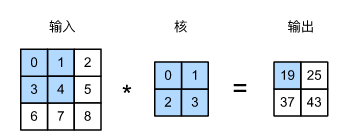
\includegraphics[width=\textwidth]{pic/Con_layer.png}
	\caption{卷积操作示意}
	\label{Con_layer}
\end{figure}

\subsection{激活层}

神经网络中的每个神经元,本层需要接受上一层的输出值作为本层神经元的输入值,并将输入值传递给下一层,输入层神经元节点会将输入属性值直接传递给下一层。因此在多层神经网络中,上层节点的输出和下层节点的输入之间存在一个函数关系,这个函数在神经网络结构中称为激活函数。而在实际运用过程中,激活函数的另一个作用就是,通过限制输出的数值范围,来使得神经网络结构的运算更简便。如图\ref{relu}所示,显示的是三种常见的激活函数,第一是RELU激活函数的数值范围在$[0, + \infty )$之间,第二是Sigmoid激活函数的数值范围为$(0,1)$,第三是Tanh激活函数的数值范围在$(-1,1)$ 之间。这三类激活函数最适合于神经卷积网络的传播过程,特别是RELU激活函数,广泛地运用在卷积神经网络的工程中。

\begin{figure}[h]
	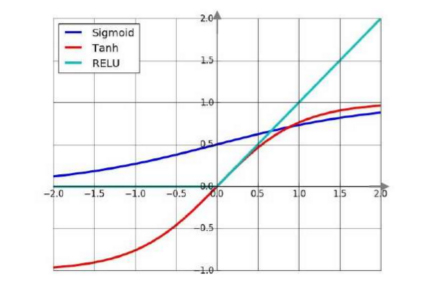
\includegraphics[width=\textwidth]{pic/relu.jpg}
	\caption{三种常见激活函数的对比示例}
	\label{relu}
\end{figure}

\subsection{池化层}

不同于卷积层就是将输入和卷积核进行互相关操作,池化层的作用则是直接计算滑动窗口内元素的最大值或者平均值,其本质其实就是降采样处理。目前学术界,对于池化而言,就是进行最大池化或者平均池化。池化层最大的优势就是在于防止出现训练过程中的过拟合问题,使得模型可以抽取更广泛的特征。

\subsection{批量归一化层}

对于浅层模型而言,标准化的预处理就已经足够满足需求啦。但是对于那些复杂的模型,当训练参数需要不断更新的时候,接近输出层的最终结果很难出现些许变化,很难训练出有效的神经网络结构。因此批归一化层的出现,就是要让这样深一点的神经网络结构的训练更加轻松容易。

在模型训练时,批量归一化计算小批量上的均值和标准差,不断调整神经网络的中间输出,从而使整个神经网络在各层的数值更稳定。

训练时,假设一个批量数据为$B = \{ {x_1},{x_2},...,{x_m}\}$,首先需要统计批量数据的的均值${\mu_B}$和方差$\sigma _B^2$,然后学习尺度参数$\gamma$和偏移参数$\beta$,将数据分布使其归一化${y_i} = \gamma \mathop {{x_i}}\limits^ \wedge   + \beta$

训练过程的计算步骤如下:
\begin{equation}
{\mu _B} = \frac{1}{m}\sum\limits_{i = 1}^m {{x_i}}
\end{equation}

\begin{equation}
\sigma _B^2 = \frac{1}{m}\sum\limits_{i = 1}^m {{{\left( {{x_i} - {\mu _B}} \right)}^2}}
\end{equation}

\begin{equation}
{\widehat x_i} = \frac{{{x_i} - {\mu _B}}}{{\sqrt {\sigma _B^2 + \varepsilon } }}
\end{equation}

\begin{equation}
{y_i} = \gamma \widehat {{x_i}} + \beta  = \gamma \frac{{{x_i} - {\mu _B}}}{{\sqrt {\sigma _B^2 + \varepsilon } }} + \beta
\end{equation}

在进行测试的环节时,因为测试样本数量较少,可以用于统计均值和方差不够用,所以需要对每批数据的期望值都要进行一定的归一化处理,测试的计算步骤如下:

\begin{equation}
E(x) = {E_B}\left[ {{\mu _B}} \right]
\end{equation}

\begin{equation}
Var[x] = \frac{m}{{m - 1}}{E_B}[{\mu _B}]
\end{equation}

\begin{equation}
y = \frac{\gamma }{{\sqrt {Var[x] + \varepsilon } }}x + (\beta  - \frac{{\gamma E(x)}}{{\sqrt {Var[x] + \varepsilon } }})
\end{equation}

\subsection{输入通道和输出通道}

对于一个图像而言,其包含的真实信息维度非常高。举个例子,彩色图像不只是只有高和宽这两个维度,实际上还包括RGB三个通道。假设高为H像素,宽为W像素,那么对于该图像而言,可以将其表示成一个3*H*W的多维数组,这第三维即叫做通道数。

在实际运用过程中,如果当输入数据1包含多个通道时,需要设计一个与输入通道数相匹配的卷积核,这样的话就能和多通道的输入数据做互相关运算啦。分析可知,输入数据的通道数为$c_i$,那么卷积核的输入通道数同样为$c_i$。设卷积核窗口尺寸为${k_h} \times {k_w}$。当${c_i} = 1$时,那么卷积核只包含一个尺寸为${k_h} \times {k_w}$	
 的二维数组。当${c_i} > 1$时,每个输入通道各分配一个尺寸为${k_h} \times {k_w}$的卷积核数组。把这$c_i$个数组在输入通道维上连结,即得到一个尺寸为${c_i} \times {k_h} \times {k_w}$的卷积核。由于输入和卷积核各有$c_i$	
 个通道,将每一个通道上的二维数组和卷积核的二维数组做互相关运算,再将这$c_i$个互相关运算的二维输出按通道相加,得到一个二维数组。
 
如图\ref{2_chan_input}所示,展示了含2个输入通道的二维互相关计算的例子。

\begin{figure}[h]
	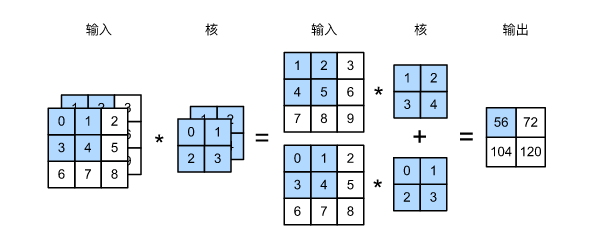
\includegraphics[width=\textwidth]{pic/2_chan_input.png}
	\caption{含2个输入通道的互相关运算}
	\label{2_chan_input}
\end{figure}

当输入通道有多个时,因为我们对各个通道的结果做了累加,所以不论输入通道数是多少,输出通道数总是为1。

\section{沙漏网络结构}

本文算法采用,沙漏网络的结构来进行人体姿态估计。该模型非常适用于人体检测任务,在MPII竞赛中获得了第一名。串联的堆叠沙漏网络复用全身关节信息,来提高对于单个关节的识别精度,后面会做进一步解释。

\subsection{残差模块}

残差模块是堆叠沙漏网络的基础模块,其原理如下:

残差网络原理如下:设输入为x,假设对于网络结构而言,理想映射为f(x)。\ref{Res_module}左图需要直接设计出该映射f(x),但是右图则需要直接设计出残差映射$f(x) \to x$。在实际情况下,残差映射更容易优化。

\begin{figure}[h]
	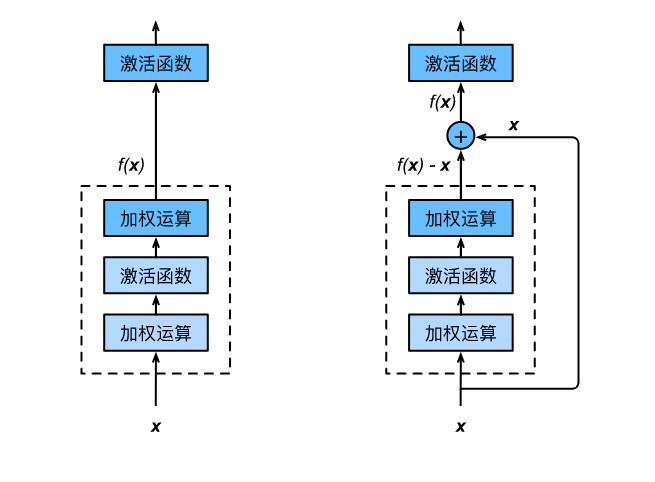
\includegraphics[width=0.8\textwidth]{pic/Res_module.jpg}
	\caption{普通的网络结构(左)与加入残差连接的网络结构(右)}
	\label{Res_module}
\end{figure}

堆叠沙漏网络结构采用了残差模块作为其基本单元,其基本结构如图所示,有主路与旁路两部分。其参数采用\citing{DBLP:journals/corr/NewellYD16}论文里设置的原始参数,这里不做更改。如图\ref{res_net}所示,主路部分上有三个尺寸分别为1*1,3*3,1*1的卷积核。旁路部分则只有一个1*1的卷积核构成,起着卷积层的作用,可以保留原始信息。然后批归一化层和激活层都作用在每一个卷积层的输入处。这也就是说,特征图在通过沙漏网络之后,并不会改变其尺寸,本质上而言,只有通道数发生了变化。

假设输入图像的通道数为M,输出图像的通道为N,则主路部分的第一个卷积层和第二个卷积层的卷积核数量都是N/2,第三个卷积层的卷积核数量为N。

其中,$M \to N$代表整个网络输入的通道数为$M$,通过网络输出的通道数转变为$N$,$w$表示设置的网络权重,$b$表示设置的偏置。

\begin{figure}[h]
	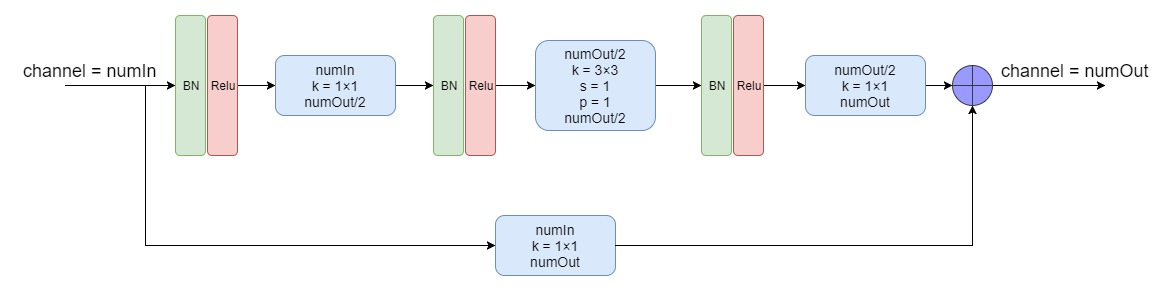
\includegraphics[width=\textwidth]{pic/res_net.jpg}
	\caption{残差模块}
	\label{res_net}
\end{figure}

\subsection{一阶沙漏网络}

\citing{DBLP:journals/corr/NewellYD16}论文介绍,一阶沙漏网络就是基于残差模块设计的,也有主路和旁路两部分,如图\ref{1_hg}所示。\citing{黄铎2019基于}对于主路部分而言,通过最大池化层,提取输入图像的特征信息并缩小图片尺寸。对于旁路而言,主要是保留输入图像的各关节点的特征信息。整体而言,使得网络在不同尺寸下的图片下都可以提取关节点的信息,而上采样可以将特征图恢复到原始尺寸,并与旁路的输出相加,最终完成提取特征的目标。输入图像提取的特征值用x来表示。其中maxpool()表示最大池化层,unsampling()表示上采样层。

\begin{equation}
y_{M \to N}^1(x) = {f_{256 \to N}}({f_{256 \to 256}}({f_{256 \to M}}(x))) + upsampling({f_{N \to N}}(...({f_{M \to 256}}(\max pool(x))))
\end{equation}

\begin{figure}[h]
	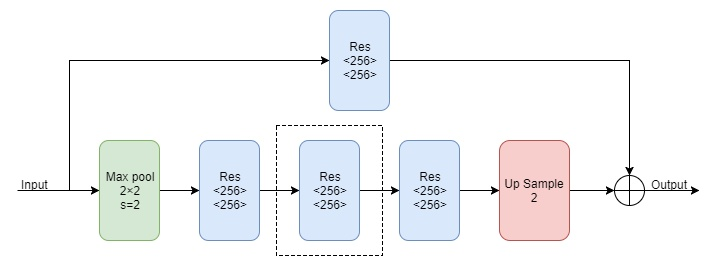
\includegraphics[width=\textwidth]{pic/1_k_hourglass.jpg}
	\caption{一阶沙漏网络}
	\label{1_hg}
\end{figure}

\subsection{二阶沙漏网络}

设计二阶沙漏网络时,只需要将一阶沙漏网络中,主路的一个残差模块替换成另一个一阶沙漏网络,如图\ref{2_hg}所示,就可以得到二阶沙漏网络。图中上下箭头分别表示上下采样,$H$和$W$分别表示输入图像的高和宽像素值,$M$和$N$分别表示整体网络输入和输处的通道数。

分析可知,在每次通过最大池化层之前,每个关节点的空间位置信息都会输入到旁路的卷积层,而且有两个残差模块来提取特征,这也就是说,二阶沙漏网络可以提取出初始,1/2,1/4尺寸的关节点特征。通过上采样使得图像尺寸恢复到与旁路相同尺寸大小,这样再进行特征融合后,即可完成目标任务。

\begin{figure}[h]
	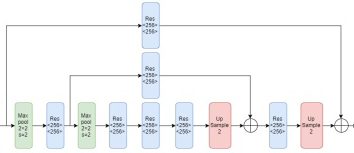
\includegraphics[width=\textwidth]{pic/2_k_hourglass.jpg}
	\caption{二阶沙漏网络}
	\label{2_hg}
\end{figure}

\subsection{四阶沙漏网络}

如法炮制,在设计四阶沙漏网络时,只需要将二阶沙漏网络中,主路的一个残差模块替换成另一个二阶沙漏网络,就可以得到一个四阶的沙漏网络。如图\ref{4_hg}所示的四阶沙漏网络。

\begin{figure}[h]
	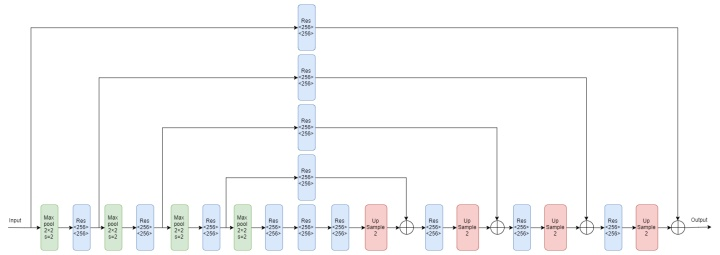
\includegraphics[width=\textwidth]{pic/4_k_hourglass.jpg}
	\caption{四阶沙漏网络}
	\label{4_hg}
\end{figure}

分析可知,对于四阶沙漏网络而言,在每次通过最大池化层之前,每个关节点的空间位置信息都会输入到旁路的卷积层,而且有两个残差模块来提取特征,这也就是说,四阶沙漏网络可以提取出初始,1/2,1/4,1/8尺寸的关节点特征。通过上采样使得图像尺寸恢复到与旁路相同尺寸大小,这样再进行特征融合后,即可完成目标任务。

\subsection{高阶沙漏网络}

本文算法采用了高阶堆叠沙漏网络作为人体姿态估计的主干检测网络。

以此类推,高阶堆叠沙漏网络在numReductions>1时,递归调用自己。

其设计的迭代思路如图\ref{8_k_hourglass}所示。

\begin{figure}[h]
	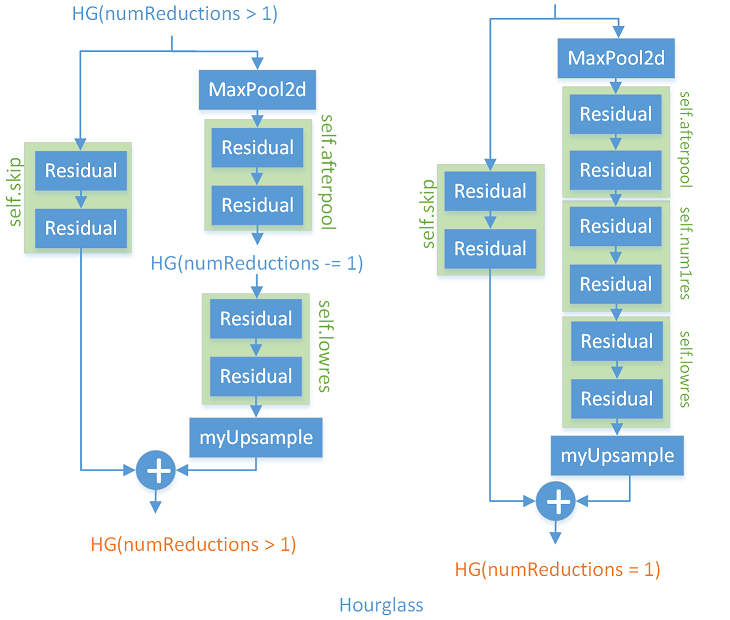
\includegraphics[width=\textwidth]{pic/8_k_hourglass.png}
	\caption{高阶沙漏网络迭代逻辑}
	\label{8_k_hourglass}
\end{figure}

\subsection{中间监督}

整个堆叠沙漏网络可以不断进行上采样和下采样的过程,\citing{DBLP:journals/corr/NewellYD16}提到这种结构的关键在于中间监督,能够对每一个沙漏模块的性能以及数据进行预测分析,在实际工程中,即在中间层级处,利用热力图计算损失。关于中间监督的位置,作者在文中也进行了讨论。对于大多数高阶特征而言,仅会在较低的分辨率下出现。如果监督再网络上采样之后,就很难在更大的全局中重新评估这些特征;如果网络能够得到最好的预测,在一个局部范围内进行的预测就很没有必要。由于沙漏网络模块整合了局部和全局的信息,若想要网络在早期进行预测,则需要它对图片有一个高层次的理解即使只是整个网络的一部分。最终,作者将中间监督设计在如下图所示位置:\ref{intermediate_supervision}

网络分裂并产生一组热力图(蓝色轮廓),其中可以应用1x1卷积,重新映射热力图,以匹配中间特征的通道数。这些是与前面沙漏模块的特征一起添加的。

\begin{figure}[h]
	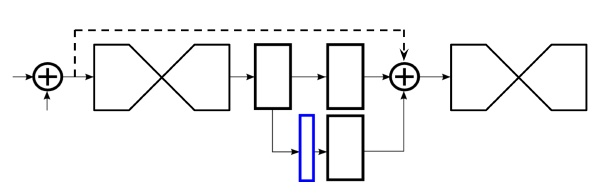
\includegraphics[width=\textwidth]{pic/intermediate_supervision.jpg}
	\caption{中间监督}
	\label{intermediate_supervision}
\end{figure}

\subsection{2D人体姿态估计算法框架的思路}

卷积神经网络的输入的图片分辨率为256×256,在沙漏网络模块中的最大分辨率为64×64,因此整个网络最开始要经过一个7×7的步长为2的卷积层,之后再经过一个残差块和最大池化层使得分辨率从256降到64。

整个算法框架只能用于单人姿态检测,但是在一张图片中经常有多个人,解决办法就是利用标签文件设计一个包围框范围,将包围框中的关节点数据判定为一个目标任务。再将目标人物裁剪到正中心后再将输入图片调整大小到256×256。整个网络使用RMSprop进行优化,学习率为2.5e-4. 测试的时候使用原图及其翻转的版本进行预测,结果取平均值。网络对于关节点的预测是热力图的最大激活值。损失函数使用均方误差(Mean Squared Error,MSE)来比较预测的heatmap与ground truth的heatmap(在节点中心周围使用2D高斯分布,标准差为1)

\begin{equation}
MSE = \frac{1}{n}\sum\limits_{i = 1}^n {{{\left( {\widehat {{x_i}} - {x_i}} \right)}^2}}
\end{equation}

\section{本章小结}
本章首先介绍了人体姿态估计中常见的深度学习技术,包括卷积神经网络各层的含义,以及输入通道和输出通道的概念。然后介绍了残差模块,沙漏模块,堆叠沙漏网络的设计原理。最后得出2D人体姿态估计算法框架的思路。
        %第二章

\chapter{人体姿态估计中的几何约束}

为了实现准确度更高的3D人体姿态估计的目标,引入几何约束可以有效地提升识别准确率,关键在于如何对人体姿态做合理化的定义。因此本章将介绍人体骨骼模型和几种常见的人体参数化表示,结合图像传感器的成像原理,介绍几个成像坐标系的转换原理。

\section{人体姿态表示}
目前在基于深度学习的3D人体姿态估计方法中常见的人体表示法有两种,一种是基于骨骼关节的点线表示法,后一种是基于固定点的姿态表示法。

\subsection{基于骨骼关节的点线表示法}

作为一种常见的人体姿态表示法,就是借助一些传感器,例如Kinect摄像头来捕捉人体三维骨骼关节点的坐标信息。就是将人体所有的关节点看作一个点,而骨骼则就是这些关节点之间的连线。至于两个点之间的角度,自由度之类的,则也可以做部分描述。这样的点线表示法,在本质上而言,就只有两个相邻的关节点才会产生一定的关联。因此在做人体姿态估计的任务时,只能够以平均关节点误差的测量指标作为衡量参数。

\subsection{基于固定点的姿态表示法}

基于固定点的关键在于,如何找到一个合适的关节点,这个关节点需要满足这个条件:其位置变化在人体整体的位置范围中是最小的。目前主要有两种形式,一种是星形结构,目前应用效果不太行,另外一种就是树形结构,能够很好地从选定好的根节点来描述人体姿态,如图~\ref{human_pose_2}所示,\citing{谢子威2019基于深度学习的}图中使用的稳定点为骨盆,对于其他关节点而言,骨盆就是汇聚的终点。

\begin{figure}[h]
	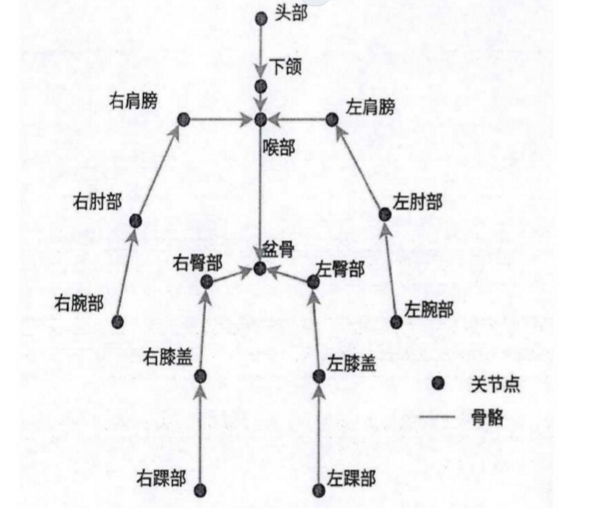
\includegraphics[width=\textwidth]{pic/human_pose_2.jpg}
	\caption{固定点表示示意图}
	\label{human_pose_2}
\end{figure}

\section{人体参数化表示}

人体姿态定义是指人体自身结构呈现的姿态,采用了树形结构\citing{陈明基于混合部件模型的姿态估计方法研究},它规定部件的位置在某个给定的根坐标下是相互独立的。从视觉上来说,用线段表示人体骨架,用点来抽象表示人体主要关节如盆骨,头,胸部,每个关节点都拥有属于各自平移和旋转的自由度,如果需要对各骨骼长度和关节角度的关系进行约束,需要借助人体解刨学的统计数据。这样一来,所有关节点的空间位置可以用以下表示。

\begin{equation}
M = \left[ {\begin{array}{*{20}{c}}
{{x_1}}&{...}&{{x_N}}\\
{{y_1}}&{...}&{{y_N}}\\
{{z_1}}&{...}&{{z_N}}
\end{array}} \right] \in {R^{N \times 3}}
\end{equation}

N为人体关节点数目。由于关键在于对人体自身姿态的分析,所以主要关注人体在三维空间中的相对姿态,在有固定关节点的位置坐标系下,基于与其他关节点之间的位置联系,重建人体三维姿态信息。

\section{误差度量}

对于人体骨骼关键点算法来说,如何有效的衡量一个算法的好坏非常重要,它不像分类问题那样可以很容易采用一些常用指标,例如precise、error、F-score等进行计算。因为在衡量的过程中,我们无法有效的将预测结果与真实值一一对应,无法知道他们之前的对应关系,更加无法知道当前的某个预测结果是否出现了误检或者漏检的情况。因此,构建一个合适的人体关键点的度量指标很重要。

\subsection{OKS}

目前最为常用的就是目标关键点相似性OKS(Object Keypoint Similarity)这个指标,启发于目标检测中的IoU指标,其目的就是为了计算真值和预测人体关键点的相似度。

\begin{equation}
OK{S_p} = \frac{{\sum {_i{e^{ - \frac{{d_{pi}^2}}{{2S_p^2\sigma _i^2}}}}\delta \left( {{v_{pi}} = 1} \right)} }}{{\sum {_i\delta \left( {{v_{pi}} = 1} \right)} }}
\end{equation}

其中:p表示真实值中人的id,I 表示关键点的id,$d_{pi}$表示真实值中每个人和预测的每个人的关键点的欧氏距离,$S_p$表示当前人的尺度因子,这个值等于此人在真实值中所占面积的平方根,即$\sqrt {\left( {{x_2} - {x_1}} \right)\left( {{y_2} - {y_1}} \right)}$,${\sigma _i}$表示第i个骨骼点的归一化因子,因此这个是通过对数据集中所有真实值计算的标准差而得到的,反映出当前骨骼点标注时候的标准差,${\sigma _i}$越大表示这个点越难标注。$v_pi$代表第p个人的第i个关键点是否可见。

\subsection{OKS矩阵}

上面介绍的OKS是计算两个人之间的骨骼点相似度的,那一张图片中有很多的人时,该怎么计算呢?这时候就是构造一个OKS矩阵了。假设一张图中,一共有M个人(groudtruth中),现在算法预测出了N个人,那么我们就构造一个M×N的矩阵,矩阵中的位置(i,j)代表groudtruth中的第i个人和算法预测出的第j个人的OKS相似度,找到矩阵中每一行的最大值,作为对应于第i个人的OKS相似度值。

\subsection{AP(平均准确率)}
此指标用于计算测试集的精度百分比,单人姿态估计和多人姿态估计的计算方式不同。

单人姿态估计,一次仅对一个行人进行估计,即在OKS指标中M=1,因此一张图片中groundtruth为一个行人(GT),对此行人进行关键点检测后会获得一组关键点(DT),最后会计算出GT与DT的相似度OKS为一个标量,然后人为的给定一个阈值T,然后可以通过所有图片的oks计算AP。即假设OKS一共有100个,其中大于阈值T的共有30个,那么AP值就是30/100=0.3.

\begin{equation}
AP = \frac{{\sum\limits_p {\delta \left( {OK{S_p} > T} \right)} }}{{\sum\limits_p 1 }}
\end{equation}

对于多人姿态估计,如果采用的检测方法是自顶向下,先把所有的人找出来再检测关键点,那么其AP计算方法如同单人姿态估计AP。如果采用的检测方法是自底向上,先把所有的关键点找出来然后再组成人,那么假设一张图片中共有M个人,预测出N个人,由于不知道预测出的N个人与groundtruth中的M个人的一一对应关系,因此需要计算groundtruth中每一个人与预测的N个人的OKS,那么可以获得一个大小为M*N的矩阵,矩阵的每一行为groundtruth中的一个人与预测结果的N个人的OKS,然后找出每一行中OKS最大的值作为当前GT的OKS。最后每一个GT行人都有一个标量OKS,然后人为的给定一个阈值T,然后可以通过所有图片中的所有行人计算AP:

\begin{equation}
AP = \frac{{\sum\limits_m {\sum\limits_p {\delta \left( {OK{S_p} > T} \right)} } }}{{\sum\limits_m {\sum\limits_p 1 } }}
\end{equation}

\subsection{PCK}

PCK(Percentage of Correct Keypoints)正确估计出的关键点比例。这是比较老的人体姿态估计指标,在2017年比较广泛使用,作为工程项目使用来评价训练的模型好坏还是蛮方便的。

\begin{equation}
PCK_i^k = \frac{{\sum\limits_p {\delta \left( {\frac{{{d_{pi}}}}{{d_p^{def}}} \le {T_k}} \right)} }}{{\sum\limits_p 1 }}
\end{equation}

其中:I表示id为i的关键点,k表示第k个阈值,p表示第p个行人,$d_pi$表示第p个人中id为i的关键点预测值与人工标注值的欧式距离。$d_p^{def}$表示第p个人的尺度因子,此因子不同公开数据集使用的计算方法不一样,FLIC数据集是以当前人的躯干直径作为尺度因子,即左肩到右臀的欧式距离或者右键到左臀的欧式距离;MPII数据集是以当前人的头部直径作为尺度因子,即头部的左上点与右下点的欧式距离,使用此尺度因子的姿态估计指标也称PCKh。$T_k$是人工设定的阈值。

\subsection{MPJPE}

MPJPE(Mean Per Joint Position Error)平均每关节位置误差,是3D人体姿态估计中最常用的评价指标,每关节的位置误差是一个关节的Groundtruth和预测值之间的欧几里德距离,该种度量方法能够在空间上直观的表现出预测值与真值之间的误差。

\begin{equation}
MPJPE = \frac{1}{T}\frac{1}{N}{\sum\limits_{t = 1}^T {\sum\limits_{i = 1}^N {\left\| {\left( {J_i^{\left( t \right)} - J_{root}^{\left( t \right)}} \right) - \left( {\widehat J_i^{\left( t \right)} - \widehat J_{root}^{\left( t \right)}} \right)} \right\|} } _2}
\end{equation}

其中T为样本数量,N为关节点的数量。计算单位为mm。

\section{人体姿态估计数据集}

对于人体姿态估计而言,目前采用的照片数据集主要分为两类:2D数据集,3D数据集

\subsection{2D数据集}

2D人体姿态识别在dataset和model方面都比3D成熟,2Dmodel也有很多户外,自然界的dataset,但是3D的dataset几乎都是室内的的。常见的数据集,如COCO,MPII。

微软团队开发了一个可以用于计算机视觉很多领域地图像数据集COCO,其全名叫做Common Objects in Context。为了满足训练,验证,测试这三流程的需要,COCO数据集中的图像也可以分为训练、验证和测试这三大类。

\begin{table}[h]
    \centering
    \begin{tabular}{c|c|c|c|c|c}
        \hline
         0-鼻子 &  1-脖子 & 2-右肩 & 3-右肘 & 4-右手腕 & 5-左肩\\
        \hline
         6-左肘 &  7-左手腕 & 8-右臀 & 9-右膝盖 & 10-右脚踝 & 11-左臀\\
        \hline
         12-左膝盖 &  13-左脚踝 & 14-右眼 & 15-左眼 & 16-右耳朵 & 17-左耳朵\\
        \hline
    \end{tabular}
    \caption{COCO标注}
    \label{COCO}
\end{table}

MPII人体姿势数据集是关节式人体姿势估计评估的最新基准。该数据集包括大约25K张图片,其中有超过40K人的身体关节有注释。这些图像是分类收集人类日常活动的。总体而言,训练集带有前后不带注释的帧。此外,对于测试集,我在研究过程中获得了更丰富的注释,包括身体部位遮挡和三维躯干和头部方向。

\begin{table}[h]
    \centering
    \begin{tabular}{c|c|c|c|c|c}
        \hline
         0-右脚踝 &  1-右膝盖 & 2-右臀 & 3-左臀 & 4-左膝盖 & 5-左脚踝\\
        \hline
         6-盆骨 &  7-胸部 & 8-上颈 & 9-头顶 & 10-右手腕 & 11-右肘\\
        \hline
         12-右肩 &  13-左肩 & 14-左肘 & 15-左手腕 \\
        \hline
    \end{tabular}
    \caption{MPII标注}
    \label{MPII}
\end{table}

\subsection{3D数据集}

在数据处理阶段,3D比2D复杂很多。2D人体姿态识别在数据集和模型方面都比3D成熟,2D模型也有很多户外,自然界的数据集,但是3D的数据集几乎都是室内的的。因为3D标注、识别的复杂,所以需要大量的传感器,摄像头去采集数据。

目前主流的3D数据集是Human3.6M,其图像是由四个摄像头捕捉完成的,分别对11个实验测试对象进行捕捉,动作类别也有60种,如\ref{human_dataset}下图所示:

\begin{figure}[h]
	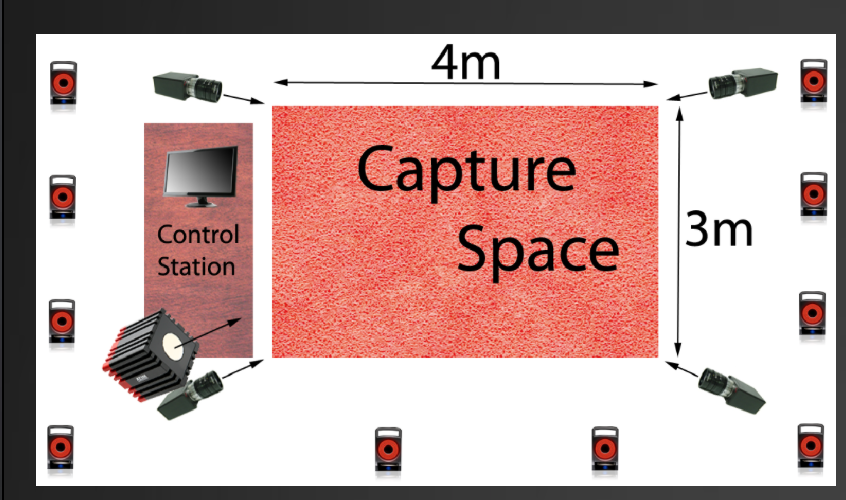
\includegraphics[width=\textwidth]{pic/human_dataset.png}
	\caption{HUMAN3.6M示意图}
	\label{human_dataset}
\end{figure}

由于需要使用该数据集,需要以一个研究机构的名义来申请,且流程极其复杂,所以在本文的研究过程中,只好采用2D数据集,来挖掘其深度信息,最终满足三维人体姿态估计的任务。

\section{成像原理}

图像成像单元在成像过程中扮演着非常重要的作用,因为需要将三维的空间信息映射到二维平面上。因此本节将会介绍,如何提取分析这一个流程的特征信息,以及如何应用于三维人体姿态估计。

\subsection{摄像机模型及其坐标系介绍}

对于一张图片而言,如何从一个三维的立体空间,经过准确的转换,可以以一个较小的信息损失来完成成像任务,这是一个研究内容。将成像流程简略表述如下,即真实物体的空间位置转换到照片成像的几何变化关系。转换过程如\ref{4_para_trans}图所示。

\begin{figure}[h]
	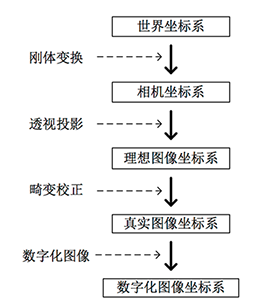
\includegraphics[height=\textwidth]{pic/4_para_trans.png}
	\caption{坐标系转换流程}
	\label{4_para_trans}
\end{figure}

摄像机成像的本质就是将三维空间信息映射到二维平面上的像素信息,而在实际情况下,世界坐标系,摄像机坐标系,成像坐标系以及图像坐标系的相关转换,需要考虑很多因素,比如摄像机的内参以及角度。世界坐标系就是标定点的位置,用毫米(mm)衡量。摄像机坐标系则以相机的光心为原点给出摄像角度的坐标位置,用毫米(mm)衡量。成像坐标系则以摄像机成像平面的坐标位置,用毫米(mm)衡量。图像坐标系则以相机拍摄图片为基准的坐标位置,用像素(mm)来衡量。

\subsubsection{刚体变换(世界坐标系与摄像机坐标系的转换)}

\citing{陈学梅2018基于人体三维姿态的动作评价系统}世界坐标系($X_w,Y_w,Z_w$),是一个三维直角坐标系,可以准确描述相机和待测物体的真实位置。

摄像机坐标系($X_c,Y_c,Z_c$),也是一个三维直角坐标系,镜头光心就是原点,x、y轴分别与相面的两边平行,z轴为镜头光轴,与像平面垂直。

世界坐标系通过旋转矩阵R和平移矩阵T转换得到摄像机坐标系,如图所示,P为空间中的点,其在世界坐标系中表示为$
P\left( {{X_w},{Y_w},{Z_w}} \right)$,在摄像机坐标系中表示$
P\left( {{X_c},{Y_c},{Z_c}} \right)$,三者的坐标系转换关系可用公式表达。

\begin{equation}
\left[ {\begin{array}{*{20}{c}}
{{X_c}}\\
{{Y_c}}\\
{{Z_c}}\\
1
\end{array}} \right] = \left[ {\begin{array}{*{20}{c}}
R&T\\
0&1
\end{array}} \right]\left[ {\begin{array}{*{20}{c}}
{{X_w}}\\
{{Y_w}}\\
{{Z_w}}\\
1
\end{array}} \right]
\end{equation}

\begin{figure}[h]
	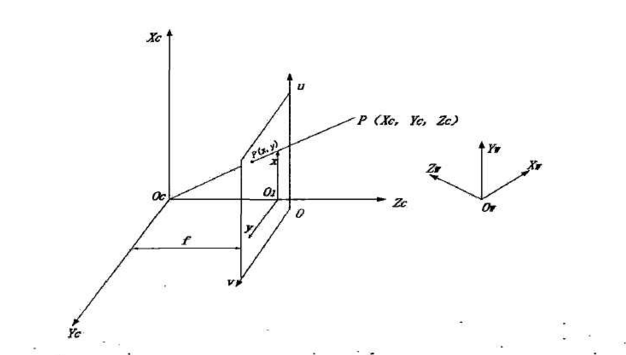
\includegraphics{pic/para_1.png}
	\caption{世界坐标系和摄像机坐标系的转换}
	\label{para_1}
\end{figure}

\subsubsection{透视投影(摄像机坐标系和成像坐标系的转换)}

其实质上就是将三维空同中的点映射成二维平面上的点,将成像平面移到相机光心与物体之间。如图\ref{para_2}所示,$O_c$为摄像机光心点,$O_1$为成像坐标系原点。由空间投影关系可得到公式:

\begin{figure}[h]
	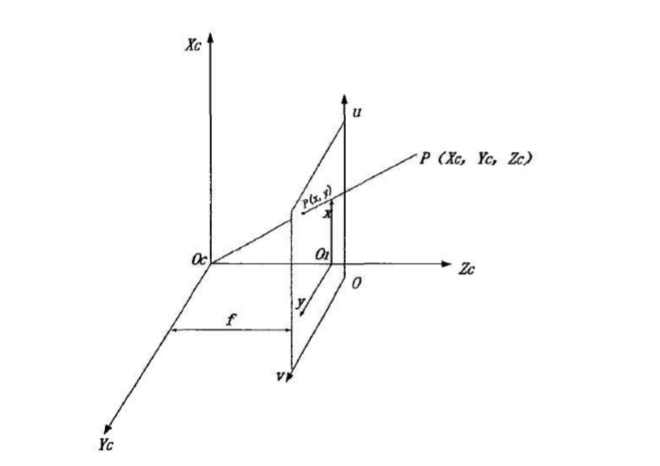
\includegraphics{pic/para_2.png}
	\caption{摄像机坐标系与成像坐标系的转换}
	\label{para_2}
\end{figure}

\begin{equation}
\left\{ {\begin{array}{*{20}{c}}
{x = f\frac{{{X_c}}}{{{Z_c}}}}\\
{y = f\frac{{{Y_c}}}{{{Z_c}}}}\\
{z = f\frac{{{X_c}}}{{{Z_c}}}}
\end{array}} \right.
\end{equation}

将上式转换为齐次坐标系表示如下:

\begin{equation}
\left[ {\begin{array}{*{20}{c}}
x\\
y\\
1
\end{array}} \right] = \left[ {\begin{array}{*{20}{c}}
f&0&0&0\\
0&f&0&0\\
0&0&1&0
\end{array}} \right]\left[ {\begin{array}{*{20}{c}}
{{X_c}}\\
{{Y_c}}\\
{{Z_c}}\\
1
\end{array}} \right]
\end{equation}

\subsubsection{二次转换(成像坐标系与图像坐标系的转换)}

成像坐标系和图像坐标系都在成像平面上,只是各自的原点和度量单位不一样。图像坐标系的原点为相机光轴与成像平面的交点,通常情况下是成像平面的中点。通过离散和平移等操作完成转换,离散化得到相应的像素位置,并且将感应到的色彩调整为用数值存储的像素信息。

\begin{figure}[h]
	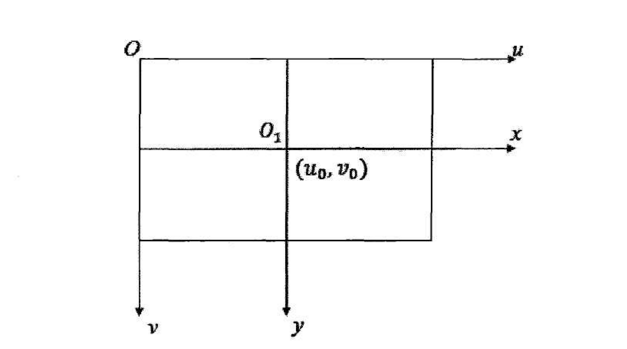
\includegraphics{pic/para_3.png}
	\caption{成像坐标系与图像坐标系的转换}
	\label{para_3}
\end{figure}

如图\ref{para_3}所示,成像坐标系的x,y轴与图像坐标系的u,v轴平行,成像坐标系的原点位于图像坐标系的(${u_0}$,${v_0}$),理想情况下该点位于图像的中心点。二者的关系可用表示:

\begin{equation}
u = \frac{x}{{dx}} + {u_0},v = \frac{y}{{dy}} + {v_0}
\end{equation}

其中dx,dy表示图像中像素间的物理尺寸,转换成齐次坐标系表示为:

\begin{equation}
{Z_c}
\left[          
  \begin{array}{c}   
    u \\
    v \\
    1
  \end{array}
\right]
=
\left[          
  \begin{array}{ccc}   
    1/dx & 0 & {u_0} \\
    0 & 1/dy & {v_0} \\
    0 & 0 & 1
  \end{array}
\right]
\left[          
  \begin{array}{cccc}   
    f & 0 & 0 & 0 \\
    0 & f & 0 & 0 \\
    0 & 0 & f & 0
  \end{array}
\right]
\left[          
  \begin{array}{cc}   
    R & T \\
    0 & 0 
  \end{array}
\right]
\left[          
  \begin{array}{c}   
    {X_w} \\
    {Y_w} \\
    {Z_w} \\
    1 
  \end{array}
\right]
\end{equation}

\begin{equation}
=
\left[          
  \begin{array}{cccc}   
    {f_x} & 0 & {u_0} & 0 \\
    0 & {f_y} & {v_0} & 0 \\
    0 & 0 & 1 & 0
  \end{array}
\right]
\left[          
  \begin{array}{cc}   
    R & T \\
    0 & 0 
  \end{array}
\right]
\left[          
  \begin{array}{c}   
    {X_w} \\
    {Y_w} \\
    {Z_w} \\
    1 
  \end{array}
\right]
\end{equation}

\begin{equation}
=
\left[          
  \begin{array}{cc}   
    M & 0
  \end{array}
\right]
\left[          
  \begin{array}{cc}   
    R & T \\
    0 & 0 
  \end{array}
\right]
\left[          
  \begin{array}{c}   
    {X_w} \\
    {Y_w} \\
    {Z_w} \\
    1 
  \end{array}
\right]
\end{equation}

其中,M为相机内参矩阵,只与相机本身结构有关,记为:

\begin{equation}
M = \left[ {\begin{array}{*{20}{c}}
{{f_x}}&0&{{u_0}}\\
0&{{f_y}}&{{v_0}}\\
0&0&1
\end{array}} \right]
\end{equation}

其中,${f_x} = \frac{f}{{dx}},{f_y} = \frac{f}{{dy}}$表示$u,v$轴的尺度因子。$
\left[ {\begin{array}{*{20}{c}}
R&T\\
0&1
\end{array}} \right]$是相机的外参矩阵,是相机在世界坐标系的位置,M的值与相机的位置摆放有关。

\section{2D热图}

传统的卷积神经网络来回归人体关键节点坐标的方法,其实并不能实现精准定位,目前的研究\cite{zhang2019distributionaware}中,采用回归热力图才能得到较高水平,这是因为热力图的本质就是概率图,图中的高斯峰值处,就是预测到的关节位置出现概率最大的位置坐标。为了使得热力图标签能和对应的目标对象不发生错乱,所以必须要分配好不同的热力图标签。

其生成公式如下:

\begin{equation}
G\left( {i,j} \right) = \frac{1}{{\sqrt {2\pi {\delta ^2}} }}{e^{\frac{{{{\left( {i - \widetilde x} \right)}^2} + {{\left( {j - \widetilde y} \right)}^2}}}{{2{\delta ^2}}}}}
\end{equation}

在这里我们假设,$i = 1,2,...,\widetilde w$,$j = 1,2,...,\widetilde h$可以表示热力图的空间位置变化,(i,j)是人体关节点的位置坐标,$ \left( {\widetilde x,\widetilde y} \right) $对应(x,y)在热力图中的位置, $ \delta $是控制高斯分布函数的参数(上图中亮斑的半径)。热力图尺寸一般小于原图尺寸,假设热力图的尺寸是原图像尺寸的1/p倍,则 $ \left( {\widetilde x,\widetilde y} \right) $人体关键点坐标也将会对应地缩小1/p倍,$ 
\left( {\widetilde w,\widetilde h} \right)$是原图尺寸(w,h)也将会缩小1/p倍。
关于人体姿态的十六个关节点的识别则根据热力图进行判断,如图\ref{heatmap}所示,显示出来亮斑的地方就是关节点概率最大的位置。

因此热力图的目标就是预测给定输入图像中的关节坐标。为此,我们需要借助之前第二章所提到的沙漏模型,在模型训练和测试期间,热力图经常被用作坐标表示。\cite{zhang2019distributionaware}具体来说,我们假设可以访问一组训练图像。为了便于模型学习,我们将标注的关节地真坐标编码成热图作为有监督的学习目标。在测试过程中,我们需要将预测的热图解码成原始图像坐标空间中的坐标。

\begin{figure}[h]
	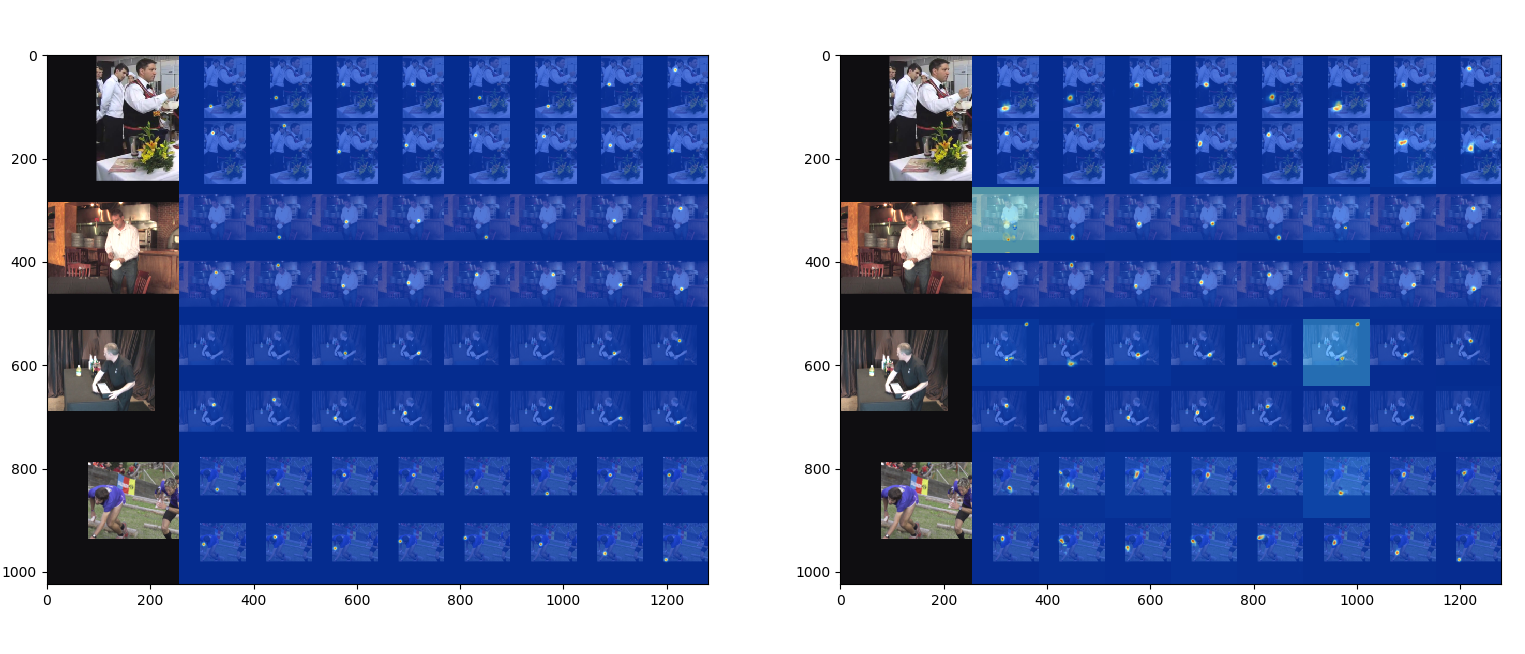
\includegraphics[width=\textwidth]{pic/screenshot.png}
	\caption{2D热力图演示}
	\label{heatmap}
\end{figure}

\section{深度回归模块}

根据一些相关文献,一般而言,2D的前两维坐标相较于而言,识别精度较高,而对于第三维坐标(Z),识别的误差较大,所以设计一款深度回归模块,用于更好地得到第三维坐标,提高3D人体姿态估计的精度。

\subsection{针孔成像原理}

对于针孔成像模型,我们这里做出如下推导。在该图中,绿色箭头和蓝色箭头分别代表以x轴和y轴为中心的关键点的坐标。而黄线代表的是射线,c代表针孔。$d,f,l_{sensor}$代表的是相机与人的关键点之间的距离(mm),焦距(mm),在图像坐标系上的人的长度(mm)。根据tan的定义,我们可以得到如下推导。

\begin{figure}[h]
	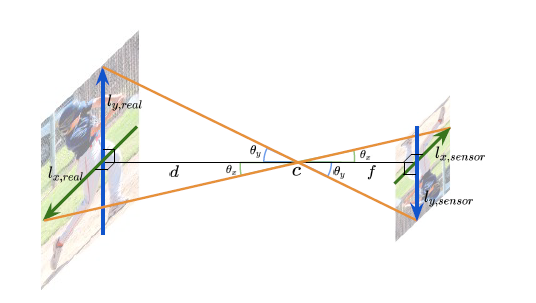
\includegraphics{pic/depth.png}
	\caption{针孔成像原理}
	\label{depth}
\end{figure}

\begin{equation}
\tan {\theta _x} = \frac{{0.5{l_{x,real}}}}{d} = \frac{{0.5{l_{x,sensor}}}}{f}
\end{equation}

其中,我们做出假设$p_x,p_y$成为指定坐标系的像素距离参数因子,然后可以得到

\begin{equation}
d = f\frac{{{l_{x,real}}}}{{{l_{x,sensor}}}} = f{p_x}\frac{{{l_{x,real}}}}{{{l_{x,sensor}}{p_x}}} = {\alpha _x}\frac{{{l_{x,real}}}}{{{l_{x,img}}}}
\end{equation}

同理可得,在y轴上也适用

\begin{equation}
d = f\frac{{{l_{y,real}}}}{{{l_{y,sensor}}}} = f{p_y}\frac{{{l_{y,real}}}}{{{l_{y,sensor}}{p_y}}} = {\alpha _y}\frac{{{l_{y,real}}}}{{{l_{y,img}}}}
\end{equation}

所以这里我们做一个假设,认为d和x,y轴的参数因子都有关系。
结合前面两个式子,可以得到,

\begin{equation}
d = \sqrt {{\alpha _x}{\alpha _y}\frac{{{l_{x,real}}}}{{{l_{x,img}}}}\frac{{{l_{y,real}}}}{{{l_{y,img}}}}}  = \sqrt {{\alpha _x}{\alpha _y}\frac{{{A_{real}}}}{{{A_{img}}}}} 
\end{equation}

其中${\alpha _x}$,${\alpha _y}$分别代表焦距在x,y轴上的像素参数,${A_{img}}$代表图片的像素大小,单位为
$pixe{l^2}$。${A_{real}}$代表真实空间中大小,单位为$mm{l^2}$。

然而,通过针孔成像的模型得到的深度值并一定是实际的深度值,这是因为,由于${A_{img}}$是通过扩展2D边界框而获得的,因此尽管与摄像机的距离相同,但其外观可能会有所不同。例如,如图\ref{depth_ambiguity}的左图所示,尽管两个人到相机的距离相同,但他们的${A_{img}}$不同。 另一方面,在某些情况下,即使距相机的距离不同,${A_{img}}$也可以相同。 例如,在图\ref{depth_ambiguity}的右图中,儿童和成人的${A_{img}}$相似,但是,儿童比成人更靠近相机。

\begin{figure}[h]
	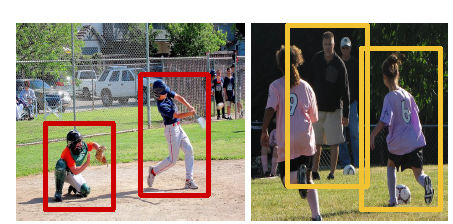
\includegraphics{pic/depth_ambiguity.png}
	\caption{深度表现的歧义性}
	\label{depth_ambiguity}
\end{figure}

根据[1]得到的图\ref{k_depth}关于d和真实的深度值的关系,呈现如下的相关性。

\begin{figure}[h]
	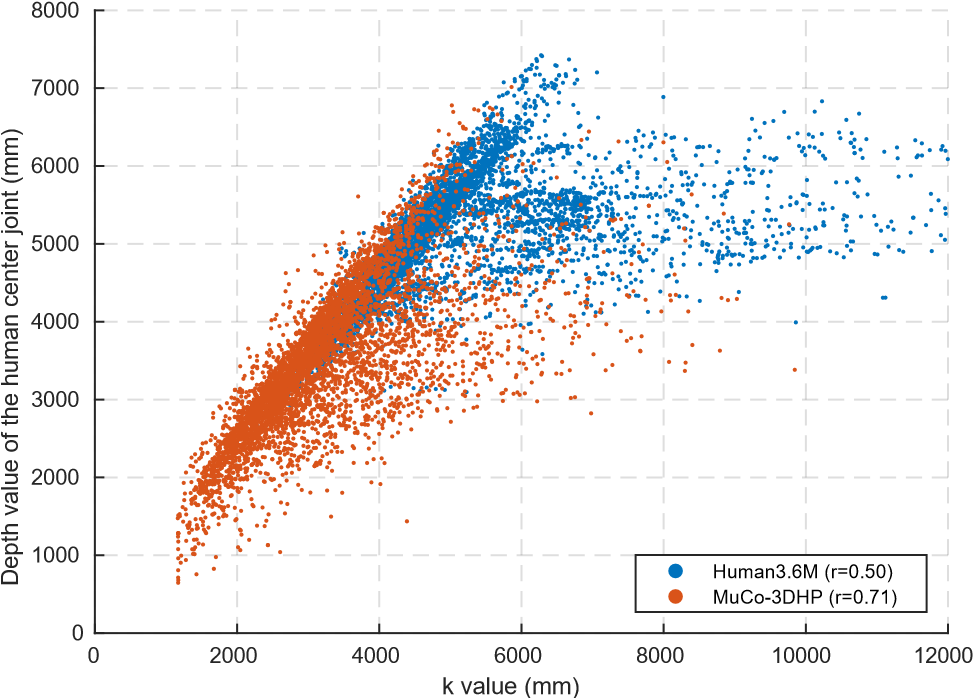
\includegraphics{pic/k_depth.png}
	\caption{k值与实际深度值的相关性。使用了人类3.6M数据集和MuCo-3DHP数据集。r表示皮尔逊相关系数。}
	\label{k_depth}
\end{figure}

为解决此问题,我们设计了矫正因子这么一个概念,以利用图像功能纠正${A_{img}}$,最终纠正d。 图像可以为深度回归提供有关${A_{img}}$必须更改多少的线索。例如,在图中\ref{depth_ambiguity},左图可以告诉深度回归增加面积,因为人类处于蹲伏状态。同样,在图\ref{depth_ambiguity}中,正确的图像可以告诉深度回归模块增加区域,因为输入图像包含一个子对象。 具体而言,深度回归模块从图像特征输出校正因子
$ \gamma$。 估计的
$ \gamma$乘以给定${A_{img}}$,即为
$ \gamma {A_{img}}$。 根据$ \gamma {A_{img}}$,计算出k,它成为最终的深度值。

结合上述的针孔成像原理,我们在这里,为简化讨论,我们设计如下模块

其算法思路如图\ref{k_depth_model}所示:

\begin{figure}[h]
	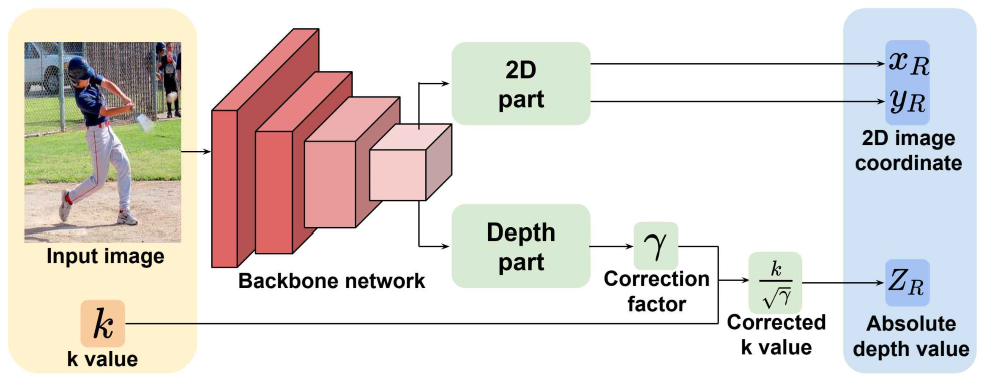
\includegraphics[width=\textwidth]{pic/K_depth_model.png}
	\caption{深度回归模块设计}
	\label{k_depth_model}
\end{figure}

网络架构包括三个组件,如图所示。首先,骨干网提取输入的人类图像的有用的全局特征。其次,二维图像坐标估计部分从骨干部分获取特征图,并使用具有批处理归一化层的三个连续卷积层和ReLU激活函数对其进行上采样。然后,1*1卷积网络被用于产生2D热图,Softargmax从2D热图提取2D图像坐标$x_R,y_R$。第三部分是深度估计部分。它还从主干部分获取特征映射,并应用全局平均池。然后,合并的特征映射经过1乘1卷积,该卷积输出单个标量值γ。最后的绝对深度值$Z_R$是通过乘以k得到的。

\section{人体姿态估计思路}

基于单目图像的三维人体识别算法按照方法可以分为两类:1.基于两阶段的三维人体姿态识别,2.基于端到端的三维人体姿态识别。

\subsection{基于两阶段的三维人体姿态识别}

基于两阶段的三维人体姿态识别,意味着计算机首先从二维RGB图像中提取人体骨架并估计其二维位置,然后根据二维骨架信息预测三维骨架的空间位置。由于二维骨架信息是三维人体姿态识别的重要输入,所以二维人体姿态识别的准确率较大地影响着三维人体识别的误差。Yang和Ramanan\citing{Yang2011}改进该模型,不采用链接式人体躯干部分,而是使用每个身体部位的混合模板来捕获部位之间的上下文共现关系,体现了局部刚性的概念。之前的工作要么使用偏离某个模板的局部可变形模型,要么在人体姿态空间中使用全局混合表示方法。

\subsection{基于端到端的三维人体姿态识别}

基于端到端的三维人体姿态识别表示在给定的图像或者视频下,将其作为输入直接输出人体骨骼关键点在三维空间中的位置。Tekin\citing{DBLP:journals/corr/TekinKSLF16}使用深度学习回归架构,用于单目图像的3D人体姿势结构化预测,该架构通过自动编码器来学习高维潜在姿态表示方法并解释关节依赖性,对人体姿态添加隐式约束。由于\citing{DBLP:journals/corr/TekinKSLF16}只是简单地将每个关节的位置误差最小化,而忽略了姿态的内部结构,Sun\citing{sun2017compositional} 使用骨骼代替关节作为姿势表示方法,并利用关节连接结构对骨骼之间的远程相互作用进行编码。Pavlakos\citing{DBLP:journals/corr/PavlakosZDD16} 为改善关节坐标的直接回归性能,首先需要对人体周围的3D空间进行离散化,
这是为了使得训练的ConvNet,可以很好地预测每个关节位置的可能性。为了自然图像中2D和3D人体姿态联合估计,Rogez\citing{8099617}提出一种用于的网络LCR-Net,不需要对图中进行近似定位,仅需在每个图像生成多个姿态提案和对其计分,最终的姿态估计是通过对相邻姿态假设进行积分而获得的。Tekin\citing{DBLP:journals/corr/TekinMSF16}为结合从图像直接回归到3D关节坐标和从2D关节位置推断3D坐标的优点,引入了判别式融合框架,以同时利用2D关节位置置信度图和3D图像提示进行3D人体姿势估计,并且提供了一种可训练的融合方案,该方案可自动学习在何处以及如何融合这两种信息源。

根据国内外研究现状所知,虽然基于两阶段的三维人体姿态识别方法在一定程度上取决于二维姿态检测器的性能,但是与基于端到端的三维人体姿态识别相比,其可以在不同的无对应关系的数据库分开训练二维、三维姿态检测器,不因只存在2D标注而无对应的3D标注的野外图像数据限制,可训练数据范围更广,训练方式更加多样化。因此,本文采用的是基于两阶段的三维人体姿态识别方法。

\section{整体算法框架设计思路}

本文算法采用两阶段的3D人体姿态估计算法,即第一步,使用骨干网络(堆叠沙漏网络)提取2D热图,根据2D热图的峰值点,即可判定于前两个坐标的最大概率位置。而第三维则采取上一节设计的深度回归模块,用来提取第三维特征,根据不同的校正因子,可以进行不同的校正作用,总之目的就是减少误差。
 
因此,整个网络架构具体设计如图所示\ref{depth_model},包括三个组件。首先,骨干网提取输入的人类图像的有用的全局特征。其次,二维图像坐标估计部分从骨干部分获取特征图,并使用具有批处理归一化层的三个连续卷积层和ReLU激活函数对其进行上采样。然后,1*1卷积网络被用于产生2D热图,Softargmax从2D热图提取2D图像坐标$x_R,y_R$。第三部分是深度估计部分。它还从主干部分获取特征映射,并应用全局平均池。然后,合并的特征映射经过1乘1卷积,该卷积输出单个标量值γ。最后的绝对深度值$Z_R$是通过乘以k得到的。

\begin{figure}[h]
	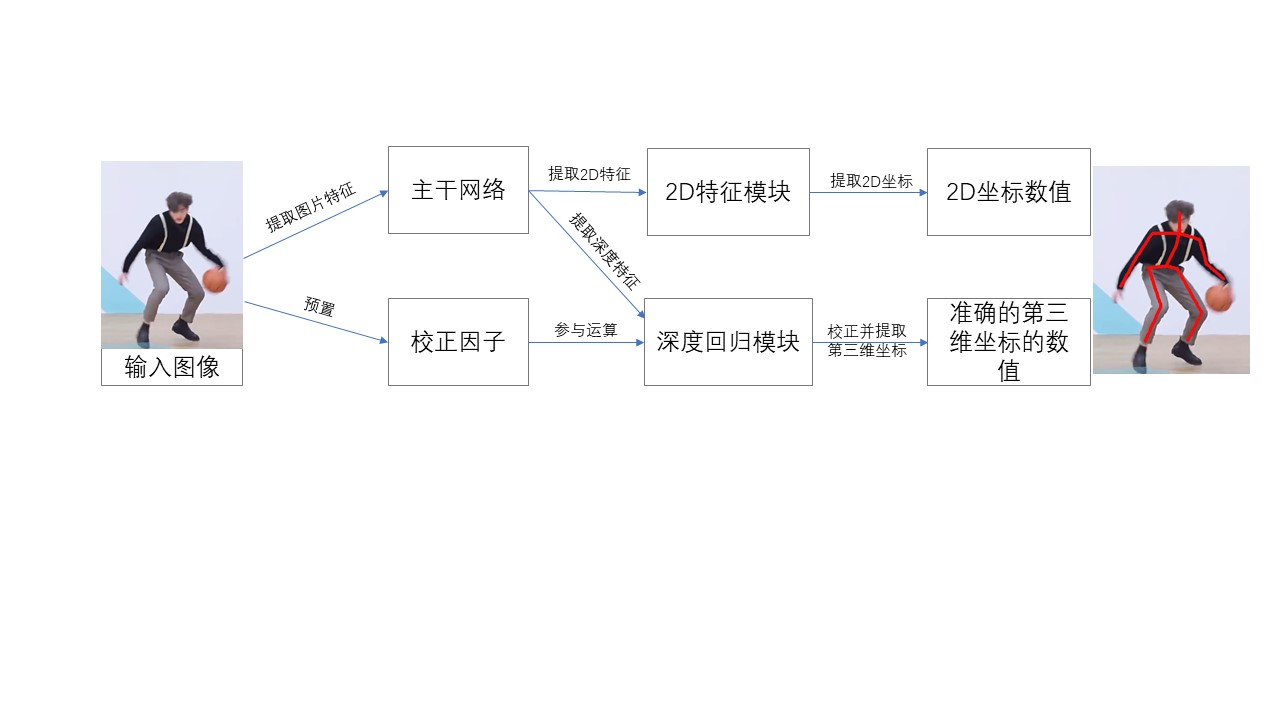
\includegraphics[width=\textwidth]{pic/depth_model.jpg}
	\caption{整体模块设计}
	\label{depth_model}
\end{figure}

\section{本章小结}
本章介绍了人体姿态估计涉及到的基本概念,并简单分析了两种常见人体姿态表示法,还有衡量人体姿态估计算法优劣的误差度量,以及目前学术界主流数据照片集的标注方法。并且介绍了摄像单元的成像原理,并结合单孔成像原理,设计了一个深度回归模块,用于提升整个算法框架。        %第三章
\chapter{三维人体姿态估计算法性能分析}

根据第二章和第三章提出的堆叠沙漏网络结构以及基于几何约束设计的深度回归模块,本章基于Ubuntu系统上进行3D人体姿态识别算法的原理性验证及性能分析。

\section{堆叠沙漏网络结构的检测算法实现}
第二章所述基于堆叠沙漏网络的人体姿态结构的识别算法,在本节中将会详细介绍其实验过程以及对应的结果分析。

\subsection{数据样本}

在进行算法实验之前,需要对数据样本做初步筛选和处理。本次实验采用MPII数据集作为实验对象,将其中约3000张照片的json信息读取出来,根据annntions文件的包围框数据,提取出对应的目标对象。随机选取其中3000个目标对象,为了使得本阶段实验的科学性。将这3000个目标对象分为两组,一组2500作为训练目标,另一组500个作为测试目标。

\subsection{堆叠沙漏网络的训练步骤}

为了探究堆叠沙漏网络的阶数对于识别效率的提升效果,进行如下实验。
本节中介绍其详细的算法实现流程及其细节。

(1)环境的搭建

整个实验是利用了GPU来进行训练,需要在ubuntu操作系统上运行,采用了python3语言以及pytorch深度学习框架。第一步是搭建显卡驱动,CUDA接口以及miniconda环境。第二步是创建一个专属本次算法实现的python虚拟环境,其中需要将python版本设置为3.6.5以上版本,并在虚拟环境中安装numpy,opencv,pytorch,torchvision等相关依赖。第三步,需要将数据集整理好,放入ubuntu系统中的设置好的工程文件。

(2)准备工作

利用opencv将数据集中的图像信息做初步特征信息的提取,设置为numpy格式,方便以后使用。将含有真实信息的annotions标记文件,按照列表的形式,也要提前读取出来。然后对图片进行数据增广,使其转化为tensor的格式,并且在BGR通道顺序改为RGB通道顺序。在设定好学习率为0.0001,批量数为20等超参数后便开始迭代训练。

在完成一次迭代过程后,选取分数最高的前100个与真实值参与损失函数的计算,完成一次迭代过程,继续下一次的迭代流程。

(3)训练实现

第一步需要将annotions文件夹中的标签文件进行处理,因为MPII数据集的标签为json格式,所以要在训练之前将所有的训练图片以及关节点数据按照列表的格式,保存在GPU的内存里。第二步则需要利用scipy对图片进行读取操作,根据标签文件的box位置,将每张图像中的多个人体目标提取出来,而且需要将尺寸设置为256*256。第三步,则根据pytorch框架的设置原则,根据骨干网路为堆叠沙漏网络的思路,还要将图像信息转化为tensor格式,设置好初始参数开始迭代训练。

每一次迭代完成以后,可以得到一个64*64*16的张量数据,根据热力图的原理,我们选取其中亮度最大的一个点,即可判断此关节点的位置就是最有可能出现的预测位置。在计算损失时,需要将得到的真实张量与真实值做比较。

4)实现人体姿态预测

在训练完成后,需要将每个关节点的预测结果中的三个坐标按照列表的形式返回,结合annotions文件的包围框的标签数据。只要是预测结果在包围框以内的关节点,即可判断这是该目标对象的关节点数据。如果预测顺利,所得到的姿态应该是16张64*64的热力图,对热力图中最亮的点进行位置信息提取,就可以得到三位预测坐标。将三维坐标信息的真实数值和预测值,做对应的评价指标的评价。
	
依次将二阶,四阶,八阶,十六阶沙漏网络进行220次迭代训练

\subsection{训练结果分析}

\begin{figure}[h]
	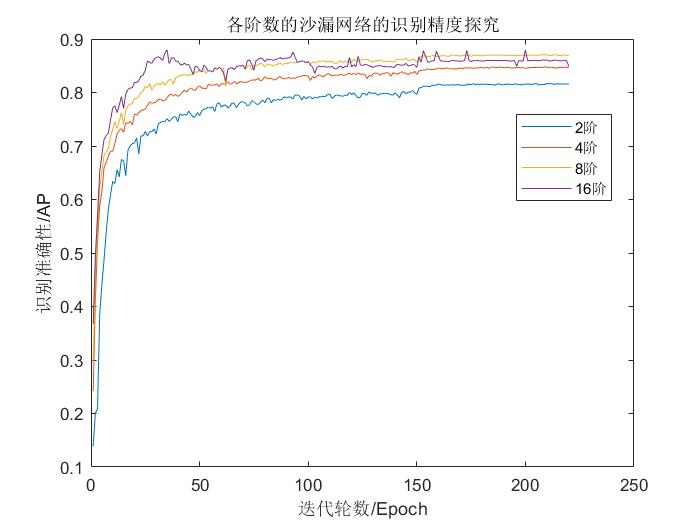
\includegraphics[width=\textwidth]{pic/stacked_hourglass.jpg}
	\caption{各阶堆叠沙漏网络的AP}
	\label{AP_graph}
\end{figure}

结合AP指标来分析,如图\ref{AP_graph}所示

可以得出以下结论:2阶到4阶的堆叠沙漏网络而言,在迭代足够多的情况下,阶数的提升提高了$3.0\%$左右的平均准确率。4阶到8阶的堆叠沙漏网络而言,在迭代足够多的情况下,阶数的提升提高了$1.6\%$左右的平均准确率。8阶到16阶的堆叠沙漏网络而言,初期迭代,识别精度提升很快,在迭代足够多的情况下,阶数的提升反而降低了$0.9\%$的平均准确率。

\begin{figure}[h]
	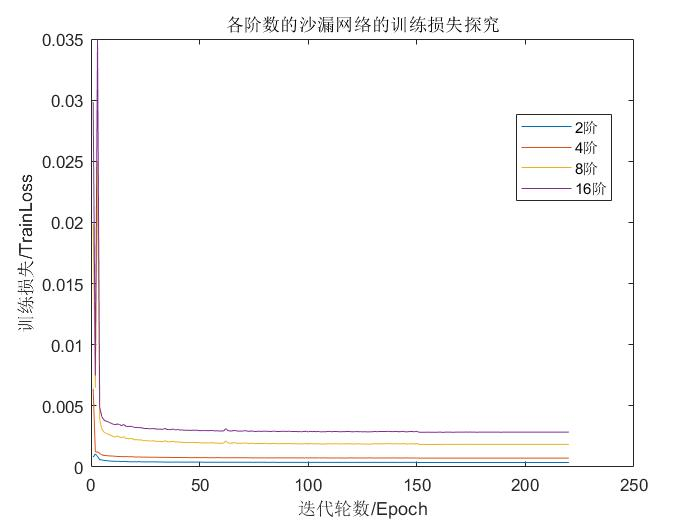
\includegraphics[width=\textwidth]{pic/stacked_hourglass_trainloss.jpg}
	\caption{各阶堆叠沙漏网络的训练误差}
	\label{Loss_graph}
\end{figure}

结合训练误差指标来分析,如图\ref{Loss_graph}所示

可以得到以下结论:训练损失曲线在前四次迭代就迅速下降后趋于平缓,几乎没有发生变化。并且随着堆叠沙漏网络阶数的提升,训练产生的损失反而更大。

总结:随着阶数的提升,确实可以提升识别准确率,但是一旦到达了一定阶数,就不能通过堆叠阶数的方式来提升识别精度,原因一,有可能是阶数过高,有可能在卷积层处理信息时,尽管有残差模块的补助,然而信息流失的概率还是很大,原因二,还有可能是,迭代到后期,在反向传播过程中,由于十六阶的网络复杂度过高,学习率的设置不太合适,导致结果过拟合。

使用MPII数据集标注的方法,结合MPJPE指标来分析。

\begin{table}[]
    \centering
    \begin{tabular}{c|c|c|c|c|c|c|c|c}
        \hline
         阶数 & Head & Shoulder	& Elbow	& Wrist	& Hip & Knee & Ankle & Mean\\
        \hline
         二阶 & 92.16 & 82.63 & 71.55 & 64.31 & 68.74 & 59.00 & 59.07 & 70.84\\
        \hline
         四阶 & 81.56 & 75.35 & 65.23 & 61.29 & 63.58 & 53.64 & 54.51 & 65.02\\
        \hline
         八阶 & 73.59 & 70.09 & 61.49 & 58.94 & 60.39 & 49.35 & 50.23 & 60.58\\
        \hline
         十六阶 & 70.25 & 68.06 & 60.56 & 57.65 & 59.49 & 50.23 & 51.56 & 59.68\\
        \hline
    \end{tabular}
    \caption{各阶堆叠沙漏网络的MPJPE}
    \label{MPII_dataset}
\end{table}

根据试验结果,可以得出以下结论:
2阶到4阶的堆叠沙漏网络而言,在迭代足够多的情况下,阶数的提升提高了5.5mm左右的平均关节误差(MPJPE)。
4阶到8阶的堆叠沙漏网络而言,在迭代足够多的情况下,阶数的提升提高了4.5mm左右的平均关节误差(MPJPE)。
8阶到16阶的堆叠沙漏网络而言,在迭代足够多的情况下,阶数的提升0.9mm的平均关节误差(MPJPE)。

总结:发现阶数的提升,确实能够带来MPJPE指标上的优化,但是到达了一定阶数,提升的效果不太明显。因为阶数越高,训练时间越久,而且效果提升不明显,所以十六阶堆叠沙漏网络的性价比不高。结合工程的实际需要,发现八阶的堆叠沙漏网络是最合适的模型,因此在本文的3D人体姿态估计算法中,最终采用了八阶堆叠沙漏网络。

\section{不同数据集的检测算法和仿真}

因为主流数据集主要有MPII,COCO,HUMAN3.6M,LSP数据集,每种数据集都有不同的标注方法,所以这里探究不同数据集对于人体姿态识别效果优劣的比较。

考虑到HUMAN3.6M的审批获取步骤很麻烦,以及LSP数据集的场景较小,因此这里只对MPII和COCO数据集进行比较。

\subsection{数据样本}

该模型的训练样本为MPII数据集与COCO数据集。其中MPII数据集信息和4.1.1一致,保持不变。对于COCO数据集而言,包含了8601张训练照片和1827张验证照片。经过上一节的分析,最终采用八阶堆叠沙漏网络,对这两个数据集中的训练图片分别进行样本分割。对于MPII训练图片而言,包含了3000个左右的目标样本。为了充分利用训练,本次实验对于MPII数据集而言,使用了2500个目标作为训练样本,500个目标作为验证样本。为了进行对比,对于COCO训练图片而言,本次实验也随机选取了2500个目标对象作为训练样本,500个目标对象作为验证样本。

\subsection{训练步骤}

为了探究不同数据集的标注方法对于识别效率的提升效果,进行如下实验。本节中介绍的算法实现的编译过程,(1)(2)(3)(4)和4.1.2基本类似,这里就不再赘述。

变动如下:(2)而训练网络中的关节点等初始化参数的设置,根据不同数据集的特点分别设置即可。(4)为方便比较不同标注方法,最后按照一个目标对象的所有关节点的位置信息,按照对应标注方法,将其映射回原始图像并且进行关节连线,即可完成人体姿态估计显示任务。

\subsection{训练结果分析}

对MPII,COCO数据集进行训练,得到训练结果如下,结合MPJPE指标来分析

\begin{table}[]
    \centering
    \begin{tabular}{c|c|c|c|c|c|c|c|c}
        \hline
         数据集 & Head & Shoulder	& Elbow	& Wrist	& Hip & Knee & Ankle & Mean\\
        \hline
         MPII & 73.59 & 70.09 & 61.49 & 58.94 & 60.39 & 49.35 & 50.23 & 60.58\\
        \hline
         COCO & 68.35 & 69.35 & 61.39 & 56.25 & 63.29 & 53.35 & 52.96 & 60.72\\
        \hline
    \end{tabular}
    \caption{MPII和COCO数据集的MPJPE}
    \label{com_dataset}
\end{table}

可以得出以下结论:
MPII数据集的标注方法,对于面部特征的标注信息较少,导致面部的几个关节点处理上不如COCO数据集。而COCO数据集,因为对面部信息的标注,使得头部的点标注误差较小。整体比较而言,数据集标注方法的差异,对于标注误差没有很大的影响,可以忽略。

训练结果图示如下:

\begin{figure}[h]
	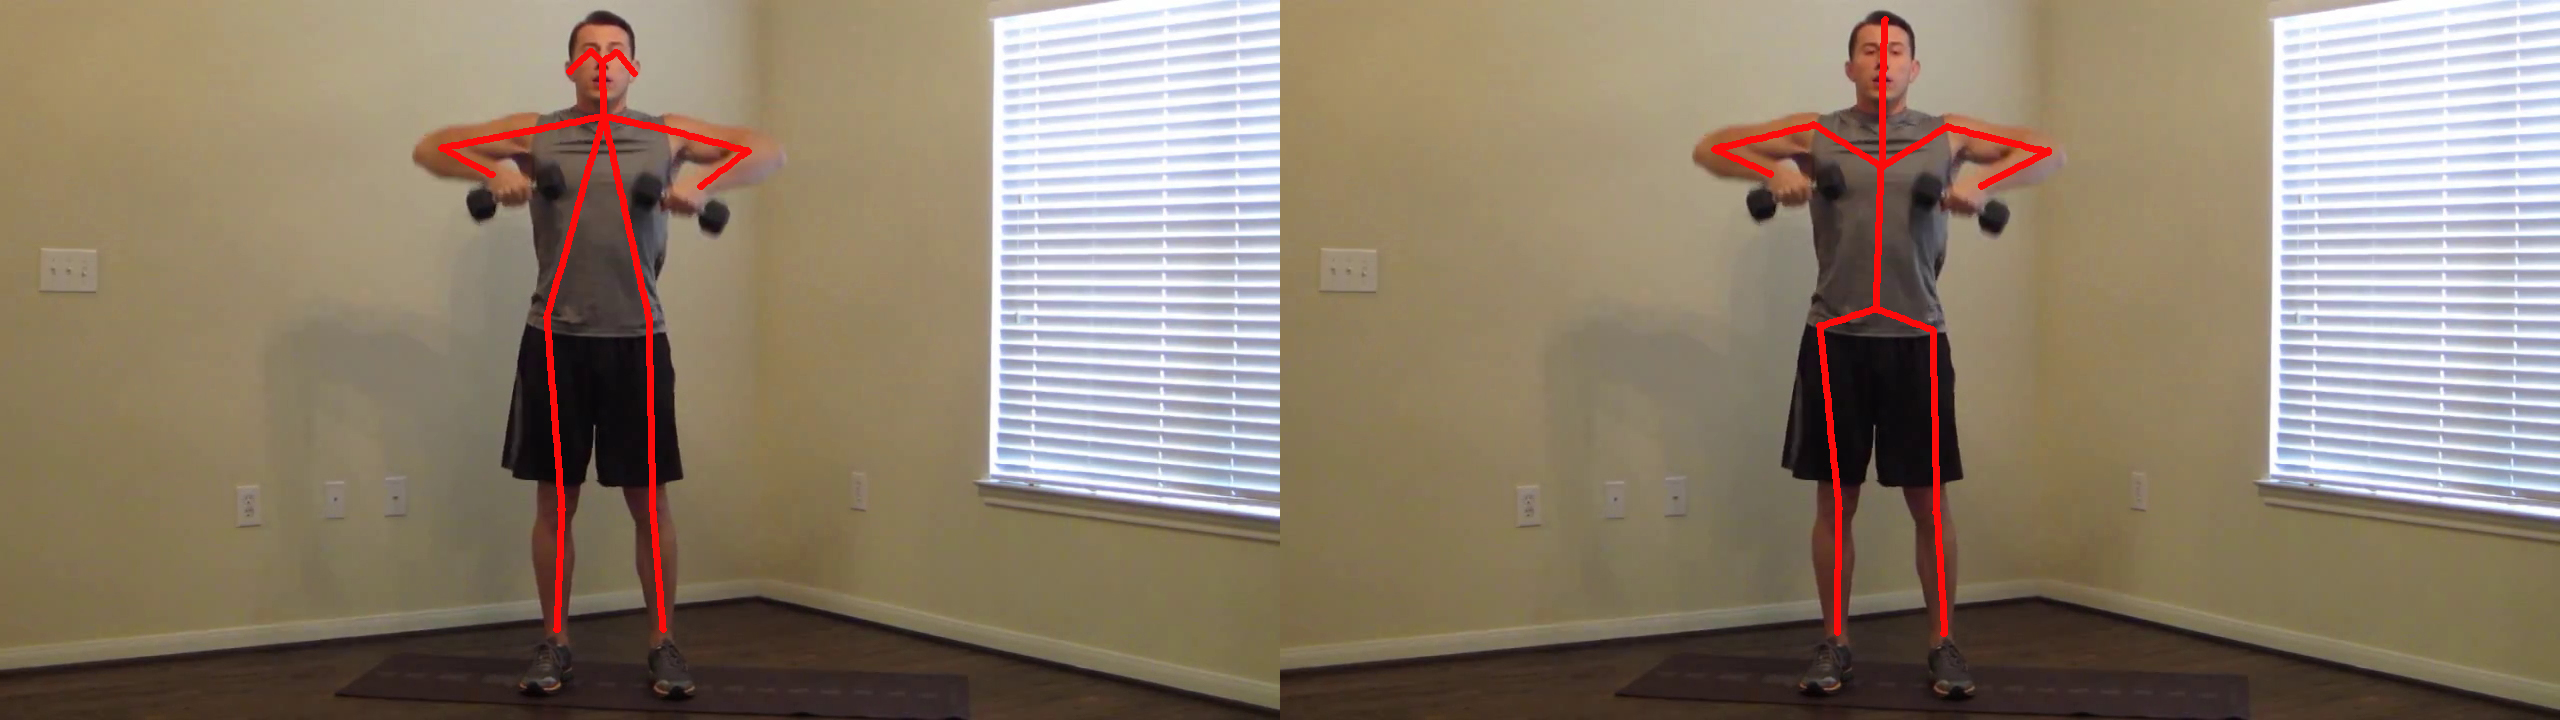
\includegraphics[width=\textwidth]{pic/vs_1.jpg}
	\caption{演示1(左图为COCO标注,右图为MPII标注)}
	\label{vs_1}
\end{figure}

\begin{figure}[h]
	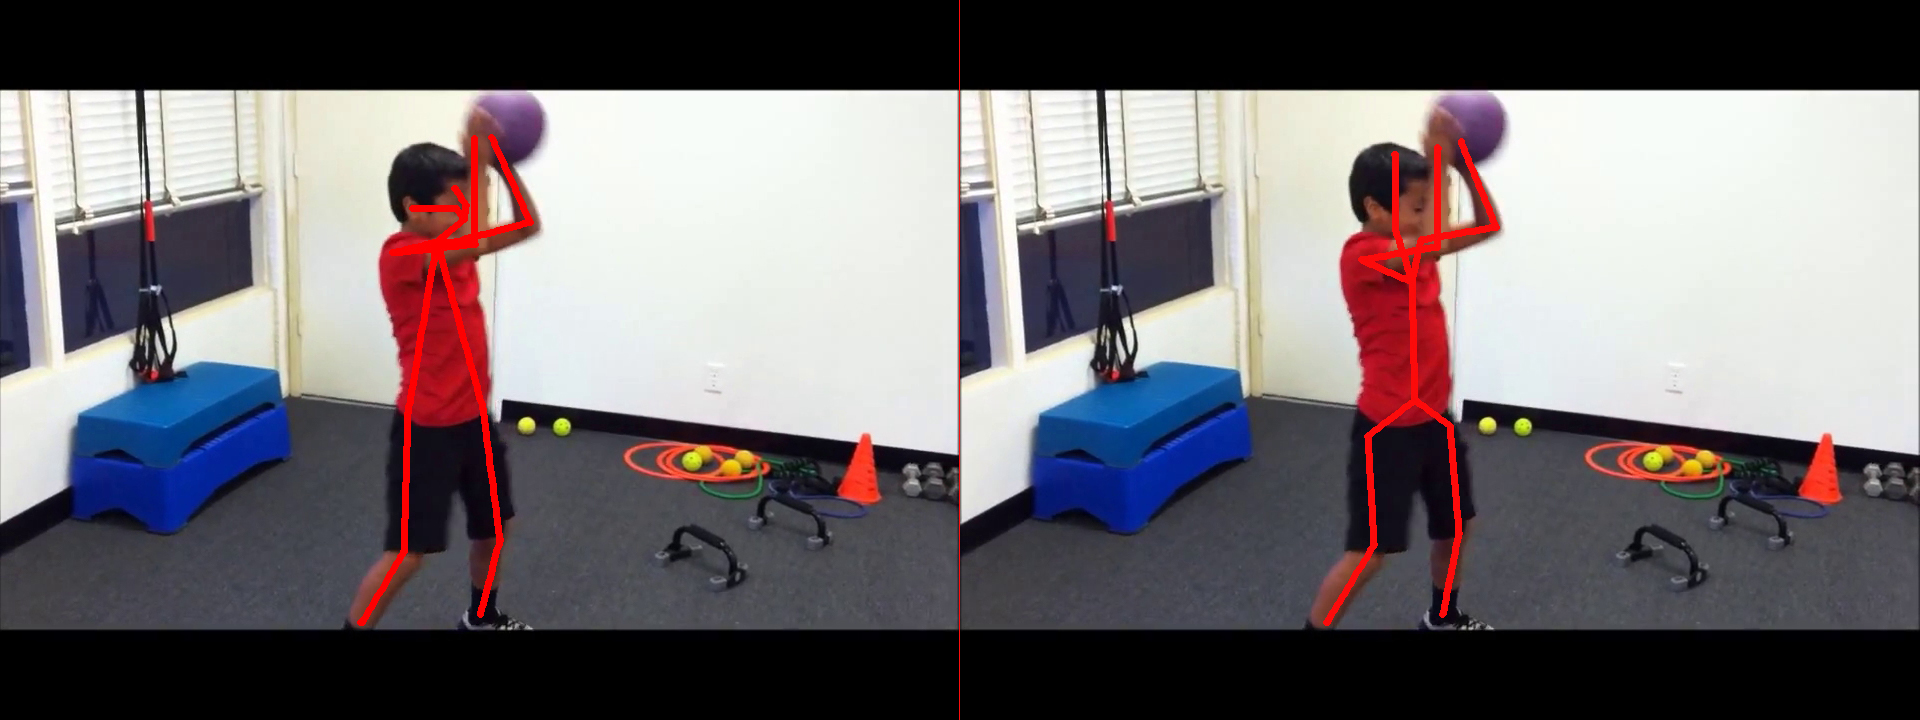
\includegraphics[width=\textwidth]{pic/vs_2.jpg}
	\caption{演示2(左图为COCO标注,右图为MPII标注)}
	\label{vs_2}
\end{figure}

因为本课题是对于人体姿态估计算法的探究,并不需要很多的面部信息标注,且数据点标注信息更多,数据集的照片数量更多,会增加项目的训练时间。因此结合工程实际需要,在后续的实验过程中,本文采用MPII数据集的标注方法,即16个关键节点即可。

\section{基于几何约束的深度回归模块的仿真}

结合第三章中介绍到的深度回归模块,我们进行了训练实验的探究。深度回归模块的仿真是建立在八阶堆叠沙漏网络的基础上的。

\subsection{数据样本}

根据annotions标签文件的包围框信息,对于MPII数据集的图片信息做初步提取,选择出之前八阶堆叠沙漏网络的3000个对象,这样提取出目标对象包围框的数据集,按照256*256的尺寸保存在GPU的内存上,等待深度回归模块的深度信息提取。

\subsection{训练步骤}

为了探究基于几何约束的深度回归模块对于识别精度的提升效果,进行如下实验。

其中骨干网,采用八阶堆叠沙漏网络,预置的参数因子,根据\citing{DBLP:journals/corr/abs-1907-11346}$\gamma$设置为0.71,步骤如下:
首先,骨干网提取输入的人类图像的有用的全局特征。其次,二维图像坐标估计部分从骨干部分获取二维特征图,并使用具有批处理归一化层的三个连续卷积层和ReLU激活函数对其进行上采样。然后,1*1卷积网络被用于产生2D热图,批归一化函数从2D热图提取2D图像坐标$X_R$,$Y_R$。第三部分是深度估计部分。它还从主干部分获取特征映射,并应用全局平均池。然后,合并的特征映射经过1乘1卷积,该卷积输出单个标量值γ。最后的绝对深度值ZR是通过乘以k得到的。

\subsection{训练结果分析}

\begin{table}[]
    \centering
    \begin{tabular}{c|c|c|c|c|c|c|c|c}
        \hline
         网络结构 & Head & Shoulder	& Elbow	& Wrist	& Hip & Knee & Ankle & Mean\\
        \hline
         初始网络 & 73.59 & 70.09 & 61.49 & 58.94 & 60.39 & 49.35 & 50.23 & 60.58\\
        \hline
         网络(深度回归模块) & 64.35 & 62.69 & 57.95 & 54.65 & 58.54 & 48.25 & 49.56 & 56.57\\
        \hline
    \end{tabular}
    \caption{MPII和COCO数据集的MPJPE}
    \label{depth_hg}
\end{table}

由于前两个坐标的识别误差并不大,据\citing{DBLP:journals/corr/abs-1907-11346}关键在于第三个坐标的误差,这个坐标在很大程度上影响整体的识别精度。根据上述结果,我们可以发现,加入深度回归模块以后,对于整个系统算法而言,识别精度得到进一步提高,约4.01mm的提升效果。这验证了设计深度回归模块的正确性以及有效性。因此本文算法最终采取了八阶堆叠沙漏网络以及深度回归模块的设计思路

\section{3D人体姿态估计算法的评价}

在MPII数据集上验证了本文算法。并且可以添加一些自己的测试数据集,以检验识别效果。只要测试数据集的人体骨盆大致位于照片中心,本文算法对一些无标注信息的照片,可以进行人体姿态估计的任务。如图\ref{vs_3}所示

\begin{figure}[h]
	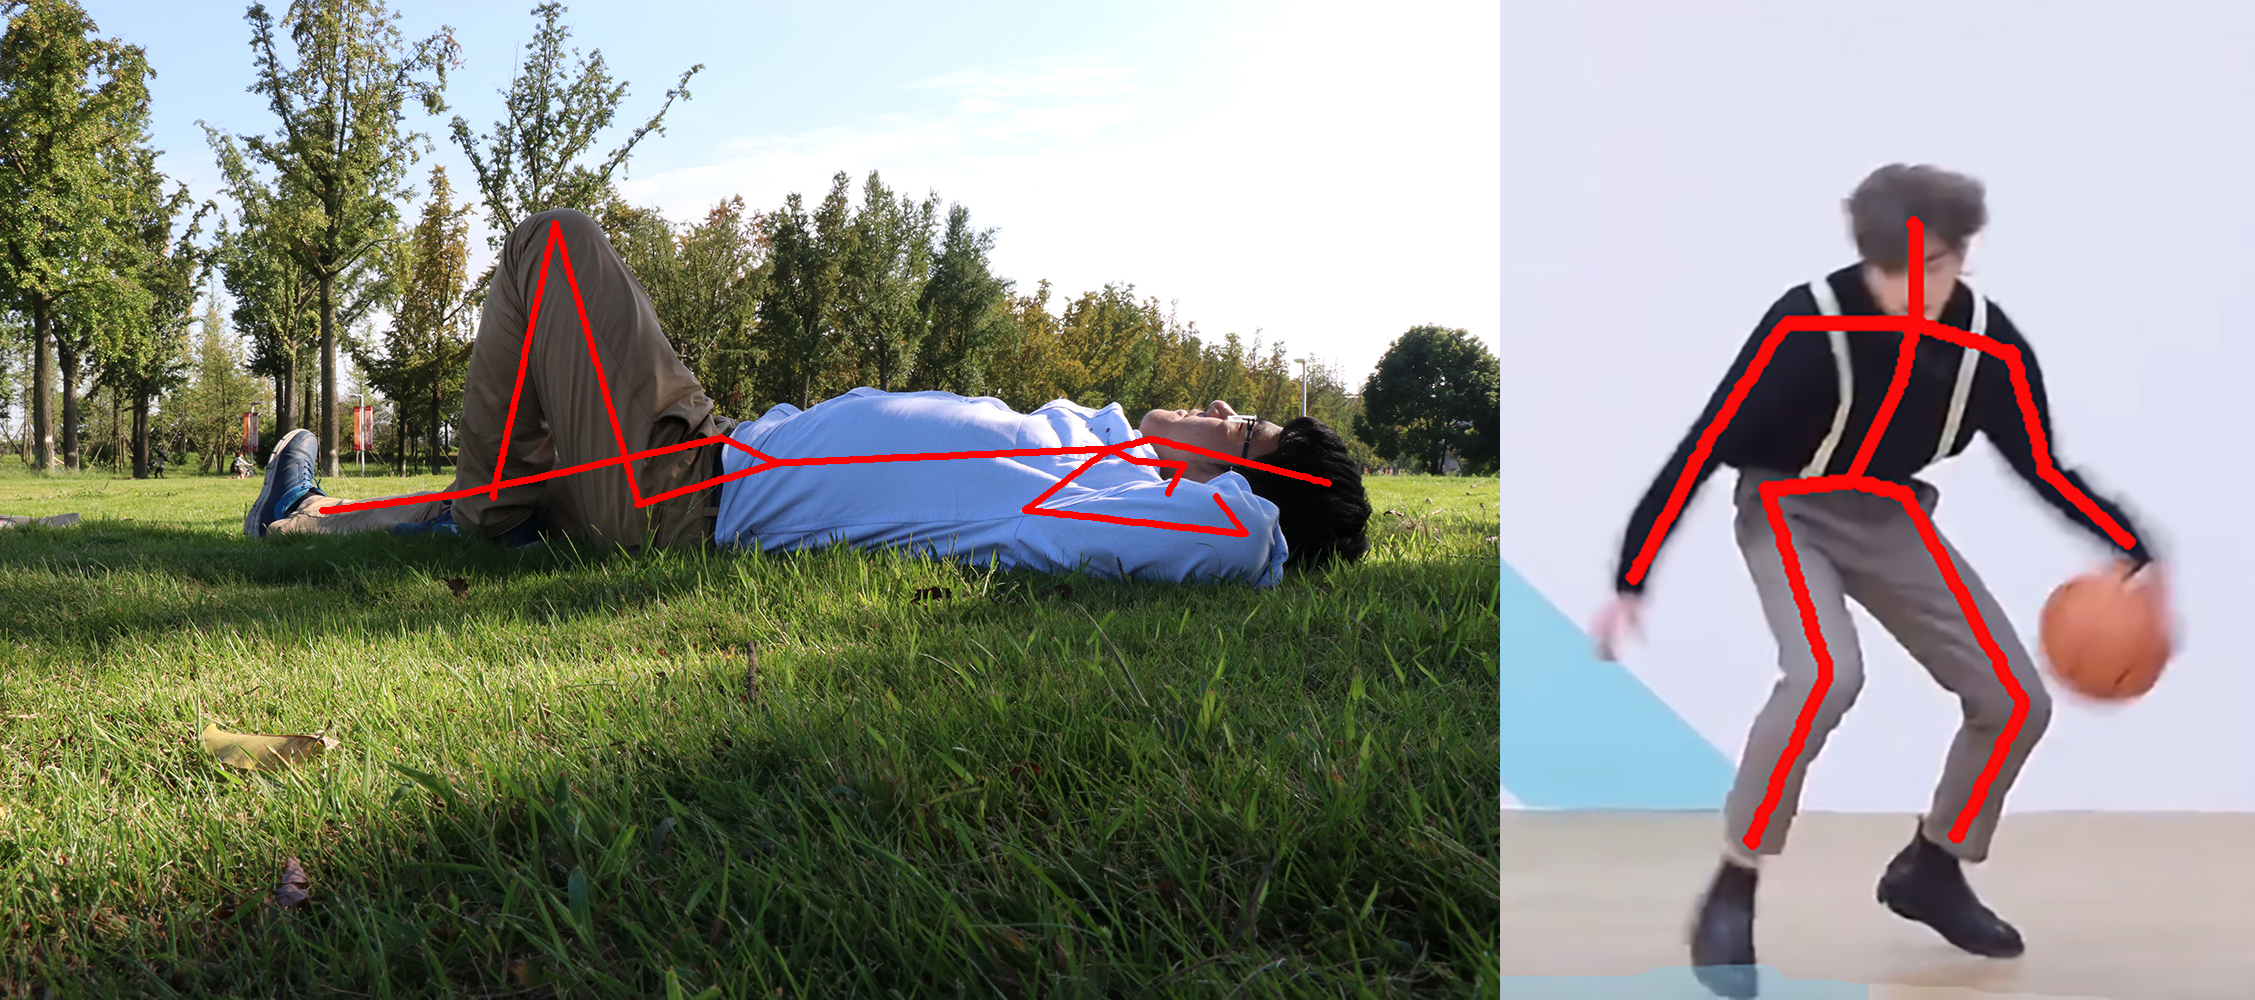
\includegraphics[width=\textwidth]{pic/vs_3.jpg}
	\caption{演示3-无标记照片}
	\label{vs_3}
\end{figure}

结果显示,整个框架算法可以精确地完成多人姿态检测任务。

\begin{figure}[h]
	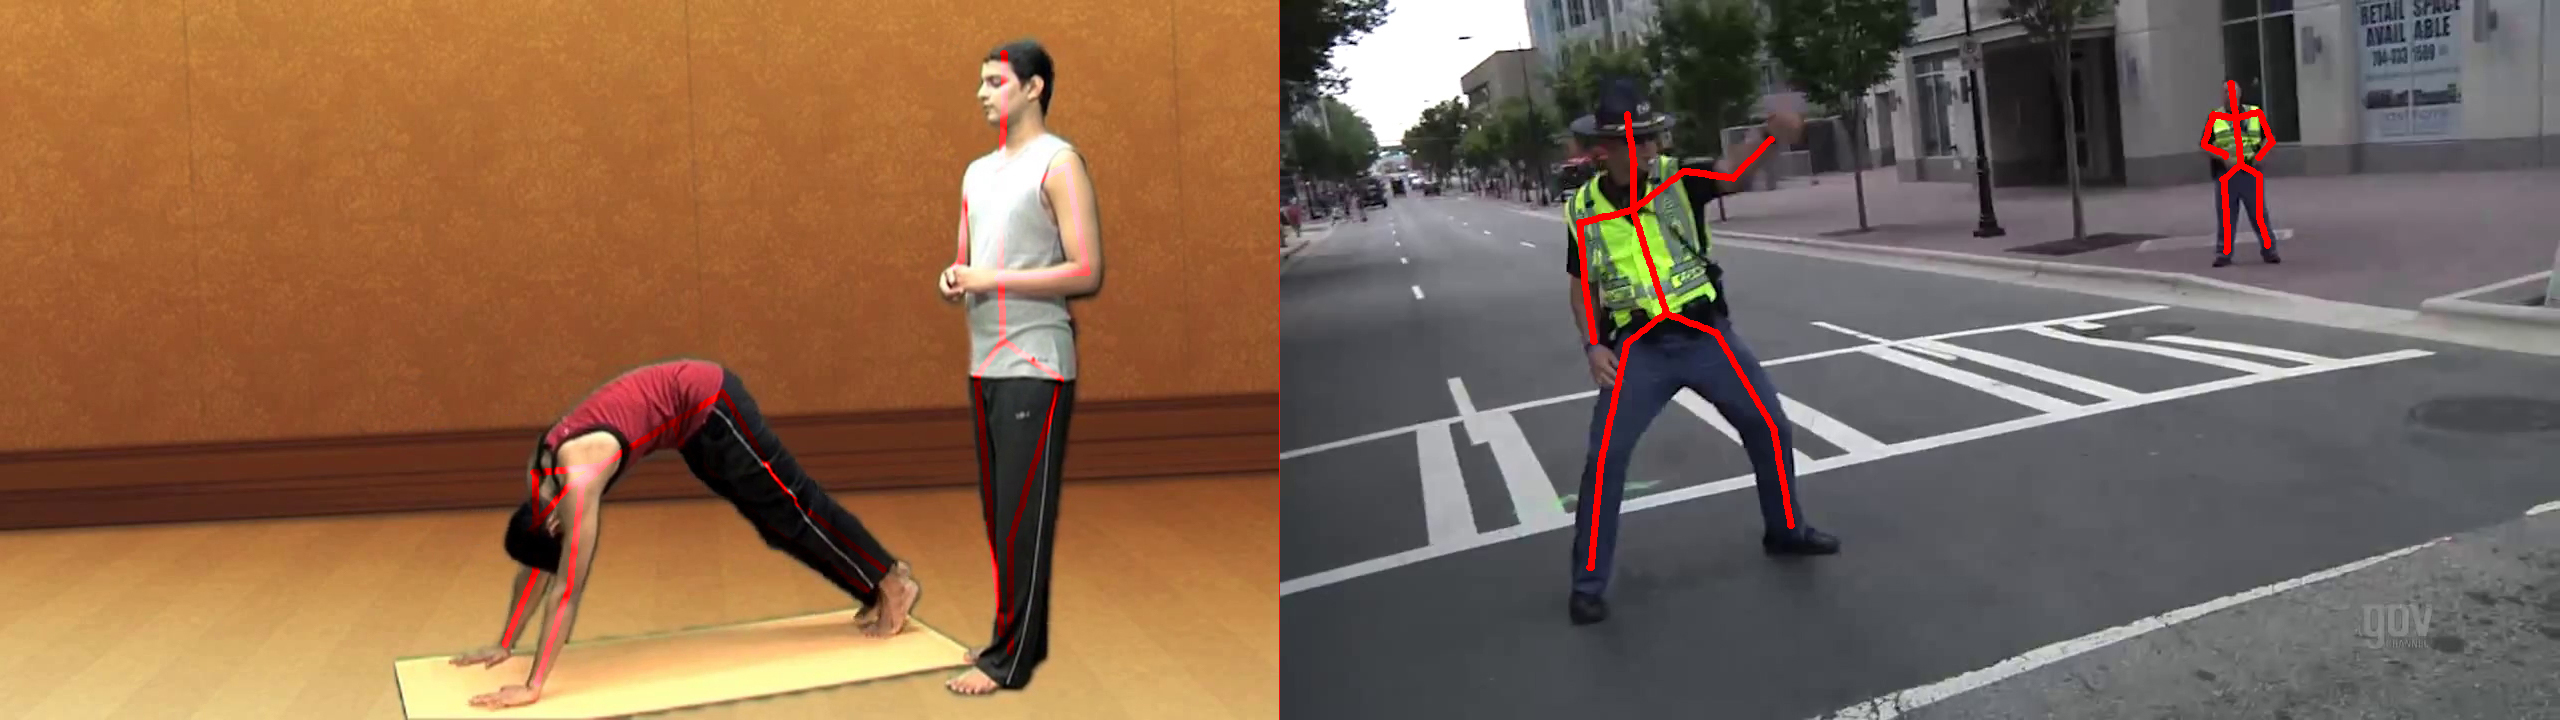
\includegraphics[width=\textwidth]{pic/vs_4.jpg}
	\caption{演示4-多人姿态检测}
	\label{vs_4}
\end{figure}

本文算法虽然在精度上有所改进,但是仍未解决传统计算机视觉中的传统问题,比如因为单目成像造成的视角局限性,导致对于一些特殊情形中的人体姿态估计出现较大误差,甚至出现歧义的情况。就比如存在一些特殊角度,在阻挡的情形下,仍然无法对某些关节点进行判断,或无法进行准确的人体姿态估计。如图\ref{error_1}所示,被测试对象的右肩膀,右肘,右手腕存在很大的误差。

\begin{figure}[h]
	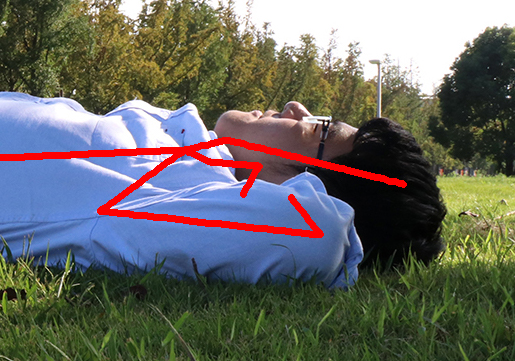
\includegraphics[height=0.6\textwidth]{pic/error_1.jpg}
	\caption{遮挡情况}
	\label{error_1}
\end{figure}

\section{本文的创新点}

1.基于人体骨骼模型,采用树形模型,采用骨盆作为人体中间点,对图像中的人体信息进行语义分割,提取出单人信息,实现多人姿态估计的任务。
2.基于沙漏模块的基础上,设计了八阶堆叠沙漏网络作为训练网络的骨干网络,使得平均关节误差MPJPE优于普通沙漏网络。
3.基于摄像成像原理,结合单孔成像,对人体姿态的第三维坐标进行了几何约束,使得第三维坐标的精确性得到了提高。
4.整体算法框架运行顺利,使得平均关节误差MPJPE达到56mm,满足任务书中的62mm的精度要求。

\section{本章小结}
本章在MPII,COCO数据集上做了实验测试,在比较各阶堆叠沙漏网络的识别效率后,得出了运算效率的最佳堆叠沙漏网络的结构。然后比较了下不同数据集的标注方法对识别效率的影响。最后,对深度回归模块的优化效果进行了验证,确实提高了识别精度。分析了整体算法的优劣,并总结本文的创新点。


        %第四章
%\chapter{全文总结与展望}

\section{全文总结}
本文以时域积分方程方法为研究背景,主要对求解时域积分方程的时间步进算法以及两层平面波快速算法进行了研究。

\section{后续工作展望}
时域积分方程方法的研究近几年发展迅速,在本文研究工作的基础上,仍有以下方向值得进一步研究:
        %第五章
%\chapter{template}
This is the template of the chapter in split file.

\section{s1}
This is a section.

\subsection{sub1}
This is a subsection. %若需添加第六章请用这个模板修改



\thesisacknowledgement
光阴似箭,转眼间我在成电的求学生涯就要结束了。在四年中,我在电子科技大学收获了很多,不局限于专业知识的学习,还锻炼了自己动手解决问题的能力,这一段学习经历,让我明白了学习是一个长期的过程,要做到终身学习和主动学习。

首先,我要感谢我的指导老师曾辽原副教授。初次认识老师是《区块链技术和应用》的课堂上,曾老师严谨负责的教学态度给我留下了深刻的映像,风趣幽默,平易近人的气质使得课堂变得异常活泼。在进行本科毕业设计期间,曾老师给予了无微不至的关怀和指导。授人以鱼不如授人以渔,教会了很多关于学习的人生哲理,并且激励我在未来的学习中要充满激情,时刻关注前沿动态。

其次,我要感谢实验室中的林吉师兄的悉心解惑。初次接触这一领域,在研习众多的论文后,我仍一头雾水,甚至无法确定思路,是师兄提出的宝贵建议,我才能确定最终解决方案。和师兄一起研究该课题过程中,师兄无私地分享了他的学术心得,帮助我快速积累了这一领域很多的知识和经验。

我还要感谢求学期间帮助过我的同学们。感谢我的室友:涂涂,志轩,老金,我们一起营造了良好的寝室氛围和环境,欢乐不断成长不停,谢谢你们对我学习和生活上的帮助。还要感谢国辉和吴巨巨,受到你们的鼓舞,组队参加了很多比赛和项目,使我锻炼了解决实际问题的能力,并且积累了自信。还要感谢班上的豪哥,老王,冠臣,能哥,虎哥,卓然,锦林,在和你们的合作中收获了信任和欢乐,我也拓宽了自己看待世界的维度。然后还要感谢大学期间结识的朋友:雷神学长,费洋学长,敏锐学姐,珉珂,辛潮,同洲,坤少,从你们的身上,看到了新一代成电人精神的传承,让我明白了什么叫做优秀。

最后,我要感谢一直默默支持,陪伴我的家人和朋友们。感谢爸妈一直以来对我的支持和关爱,用最大努力给我创造了安心舒适的学习环境,你们是我前进的动力源泉。想感谢的人太多太多,谢谢你们!
  %致谢


%\nocite{*}
\thesisbibliography{reference} %参考文献


\thesistranslationchinese
\section{堆叠沙漏网络架构}

\subsection{沙漏设计}

沙漏的设计是由需要捕捉每一个尺度上的信息驱动的。虽然局部证据对于识别面部和手部等特征至关重要,但最终的姿势估计需要对全身有连贯的理解。人的方位、四肢的排列以及相邻关节之间的关系是在图像中不同尺度下最容易识别的线索之一。沙漏是一个简单,最小的设计,有能力捕捉所有这些特征,并将它们结合起来,输出像素级的预测。 

网络必须具有某种机制,以便跨规模有效地处理和整合功能。一些方法通过使用单独的管道来解决这个问题,这些管道在多个分辨率下独立处理图像,然后在网络中组合特征[15,18]。相反,我们选择使用带有跳过层的单个管道来保留每个分辨率的空间信息。该网络以 4x4 像素的分辨率达到最低,允许应用更小的空间过滤器来比较图像整个空间的特征。 

沙漏的设置如下:卷积层和最大池层用于将特征处理到非常低的分辨率。在每一个最大池步骤,网络分支并在原始预池分辨率下应用更多的卷积。在达到最低分辨率后,网络开始自上而下的跨尺度上采样和特征组合序列。为了将两个相邻分辨率的信息汇集在一起,我们遵循汤普森等人描述的过程。[15]并对较低分辨率进行近邻上采样,然后对两组特征进行元素相加。沙漏的拓扑结构是对称的,所以在向下的每一层都有一个对应的层向上。 

在达到网络的输出分辨率后,应用连续两轮1x1卷积来产生最终的网络预测。网络的输出是一组热图,其中对于给定的热图,网络预测每个像素处存在关节的概率。完整的模块(不包括最后的 1x1 层)如图 3 所示。

\subsection{分层实施}

在保持整体沙漏形状的同时,层的具体实现仍有一定的灵活性。不同的选择会对网络的最终性能和培训产生适度的影响。我们探讨了在我们的网络层设计的几种选择。最近的工作已经显示了使用1x1卷积的简化步骤的价值,以及使用连续的较小滤波器捕获较大空间上下文的好处。[12,14]例如,可以用两个单独的3x3过滤器替换5x5过滤器。我们测试了我们的整体网络设计,根据这些见解在不同的层模块中交换。在从带有大滤波器的标准卷积层切换到像He等人提出的剩余学习模块这样的新方法之后,我们经历了网络性能的提高。[14] 以及基于“盗梦空间”的设计[12]。在使用这些类型的设计改进了最初的性能之后,对层进行的各种额外的探索和修改对进一步提高性能或训练时间几乎没有什么帮助。 

左图:我们在整个网络中使用的剩余模块[14]。右图:中间监督过程示意图。网络分裂并产生一组热图(蓝色轮廓),其中可以应用损耗。1x1卷积重新映射热图,以匹配中间特征的通道数。这些是与前面沙漏的特征一起添加的。 

我们的最终设计充分利用了残差模块。从不使用大于3x3的筛选器,并且瓶颈限制了每一层的参数总数,从而减少了总内存使用量。我们网络中使用的模块如图4所示。为了将其放到整个网络设计的上下文中,图 3 中的每个框表示一个单独的残差模块。 

以256x256 的完全输入分辨率运行需要大量的GPU内存,因此沙漏的最高分辨率(因此最终输出分辨率)为 64x64。这不会影响网络产生精确联合预测的能力。整个网络从一个7x7 卷积层开始,步长为 2,接着是一个剩余模块和一轮最大池,将分辨率从 256 降到 64。图 3 所示的沙漏之前有两个后续的残差模块。在整个沙漏中,所有残差模块输出 256 个特征。 




\thesistranslationoriginal
\section{Stacked Hourglass Network Architecture}

\subsection{Hourglass Design}

The design of the hourglass is motivated by the need to capture information at every scale. While local evidence is essential for identifying features like faces and hands, a final pose estimate requires a coherent understanding of the full body. The person’s orientation, the arrangement of their limbs, and the relationships of adjacent joints are among the many cues that are best recognized at different scales in the image. The hourglass is a simple, minimal design that has the capacity to capture all of these features and bring them together to output pixel-wise predictions.

The network must have some mechanism to effectively process and consolidate features across scales. Some approaches tackle this with the use of separate pipelines that process the image independently at multiple resolutions and combine features later on in the network [15,18]. Instead, we choose to use a single pipeline with skip layers to preserve spatial information at each resolution. The network reaches its lowest resolution at 4x4 pixels allowing smaller spatial filters to be applied that compare features across the entire space of the image.

The hourglass is set up as follows: Convolutional and max pooling layers are used to process features down to a very low resolution. At each max pooling step, the network branches off and applies more convolutions at the original pre-pooled resolution. After reaching the lowest resolution, the network begins the top-down sequence of upsampling and combination of features across scales. To bring together information across two adjacent resolutions, we follow the process described by Tompson et al. [15] and do nearest neighbor upsampling of the lower resolution followed by an elementwise addition of the two sets of features. The topology of the hourglass is symmetric, so for every layer present on the way down there is a corresponding layer going up.

After reaching the output resolution of the network, two consecutive rounds of 1x1 convolutions are applied to produce the final network predictions. The output of the network is a set of heatmaps where for a given heatmap the network predicts the probability of a joint’s presence at each and every pixel. The full module (excluding the final 1x1 layers) is illustrated in Figure 3.

\subsection{Layer Implementation}

While maintaining the overall hourglass shape, there is still some flexibility in the specific implementation of layers. Different choices can have a moderate impact on the final performance and training of the network. We explore several options for layer design in our network. Recent work has shown the value of reduction steps with 1x1 convolutions, as well as the benefits of using consecutive smaller filters to capture a larger spatial context. [12,14] For example, one can replace a 5x5 filter with two separate 3x3 filters. We tested our overall network design, swapping in different layer modules based off of these insights. We experienced an increase in network performance after switching from standard convolutional layers with large filters and no reduction steps to newer methods like the residual learning modules presented by He et al. [14] and “Inception”-based designs [12]. After the initial performance improvement with these types of designs, various additional explorations and modifications to the layers did little to further boost performance or training time.

Our final design makes extensive use of residual modules. Filters greater than 3x3 are never used, and the bottlenecking restricts the total number of parameters at each layer curtailing total memory usage. The module used in our network is shown in Figure 4. To put this into the context of the full network design, each box in Figure 3 represents a single residual module.

Operating at the full input resolution of 256x256 requires a significant amount of GPU memory, so the highest resolution of the hourglass (and thus the final output resolution) is 64x64. This does not affect the network’s ability to produce precise joint predictions. The full network starts with a 7x7 convolutional layer with stride 2, followed by a residual module and a round of max pooling to bring the resolution down from 256 to 64. Two subsequent residual modules precede the hourglass shown in Figure 3. Across the entire hourglass all residual modules output 256 features.



%
\thesisappendix

\chapter{中心极限定理的证明}

\section{高斯分布和伯努利实验}   %附录,论文若无附录则用%将该命令取消



%\thesisaccomplish{publications} %攻读学位期间取得的成果,若无成果则用%将该命令取消


\end{document}
